\documentclass[12pt]{article}
\usepackage[letterpaper, top=17mm, bottom=16mm, left=13mm, right=13mm, headheight=15pt, headsep=4mm, footskip=8mm]{geometry}
\usepackage[T1]{fontenc}
\usepackage{helvet}
\renewcommand{\familydefault}{\sfdefault}
\usepackage{tikz}
\usetikzlibrary{arrows.meta, decorations.markings}
\tikzset{midarrow/.style={postaction={decorate}, decoration={markings, mark=at position 0.5 with {\arrow{Stealth[length=3.6mm, width=3.2mm]}}}}}
\tikzset{smallarrow/.style={postaction={decorate}, decoration={markings, mark=at position 0.5 with {\arrow{Stealth[length=2.6mm, width=2.3mm]}}}}}
\tikzset{bigarrow/.style={-{Stealth[length=3mm, width=2.6mm]}, line width=1.1pt}}
\usepackage{fancyhdr}
\pagestyle{fancy}
\fancyhf{}
\lhead{\normalsize Week 62 / Conflict networks / Grades 2--3}
\lfoot{\small Bellingham Math Circle / Week 62 / W62-RV-M-v1}
\rfoot{\small \thepage}
\renewcommand{\headrulewidth}{0pt}
\setlength{\parindent}{0pt}
\setlength{\parskip}{0pt}
\raggedright
\begin{document}
\noindent\begin{minipage}[c]{0.64\linewidth}\raggedright The headers show which colour goes with each number. Put one counter on each circle. Two circles joined by a line must not get the same number. When numbers are printed next to a circle, its counter must be one of them.\end{minipage}\hfill\begin{minipage}[c]{0.33\linewidth}\raggedleft 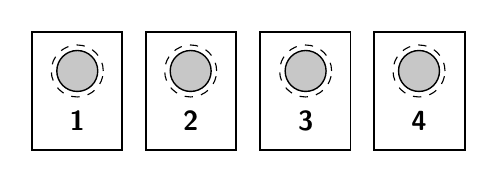
\begin{tikzpicture}[x=1mm, y=1mm]
\useasboundingbox (-0.5,-0.5) rectangle (55.5,15.5);
\draw[line width=0.7pt, fill=white] (0.0,0.0) rectangle (11.5,15.0);
\draw[dashed, line width=0.4pt] (5.8,10.0) circle (3.3mm);
\draw[line width=0.5pt, fill=black!22] (5.8,10.0) circle (2.6mm);
\node[font=\bfseries] at (5.8,3.6) {1};
\draw[line width=0.7pt, fill=white] (14.5,0.0) rectangle (26.0,15.0);
\draw[dashed, line width=0.4pt] (20.2,10.0) circle (3.3mm);
\draw[line width=0.5pt, fill=black!22] (20.2,10.0) circle (2.6mm);
\node[font=\bfseries] at (20.2,3.6) {2};
\draw[line width=0.7pt, fill=white] (29.0,0.0) rectangle (40.5,15.0);
\draw[dashed, line width=0.4pt] (34.8,10.0) circle (3.3mm);
\draw[line width=0.5pt, fill=black!22] (34.8,10.0) circle (2.6mm);
\node[font=\bfseries] at (34.8,3.6) {3};
\draw[line width=0.7pt, fill=white] (43.5,0.0) rectangle (55.0,15.0);
\draw[dashed, line width=0.4pt] (49.2,10.0) circle (3.3mm);
\draw[line width=0.5pt, fill=black!22] (49.2,10.0) circle (2.6mm);
\node[font=\bfseries] at (49.2,3.6) {4};
\end{tikzpicture}\end{minipage}\par
\vspace{4mm}
\noindent\makebox[\linewidth][c]{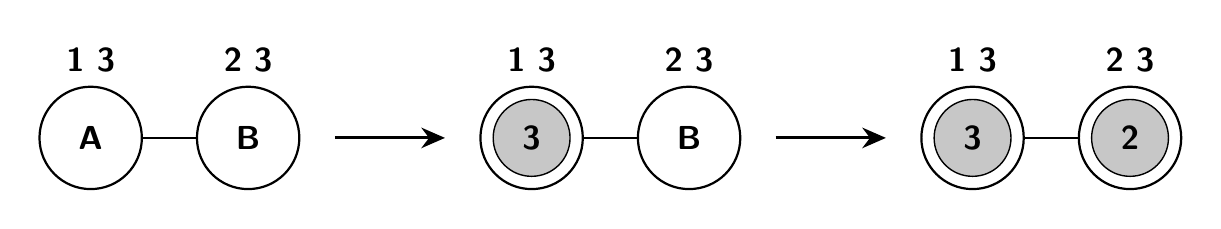
\begin{tikzpicture}[x=1mm, y=1mm]
\useasboundingbox (-8.0,-8.0) rectangle (140.0,14.0);
\draw[line width=0.8pt] (0.00,0.00) -- (20.00,0.00);
\draw[line width=0.8pt, fill=white] (0.00,0.00) circle (6.5mm);
\node[font=\large\bfseries] at (0.00,0.00) {A};
\draw[line width=0.8pt, fill=white] (20.00,0.00) circle (6.5mm);
\node[font=\large\bfseries] at (20.00,0.00) {B};
\node[font=\large\bfseries, inner sep=0.5mm, anchor=270] at (0.00,7.90) {1\,\,3};
\node[font=\large\bfseries, inner sep=0.5mm, anchor=270] at (20.00,7.90) {2\,\,3};
\draw[bigarrow] (31.0,0) -- (45.0,0);
\draw[line width=0.8pt] (56.00,0.00) -- (76.00,0.00);
\draw[line width=0.8pt, fill=white] (56.00,0.00) circle (6.5mm);
\draw[line width=0.5pt, fill=black!22] (56.00,0.00) circle (4.88mm);
\node[font=\large\bfseries] at (56.00,0.00) {3};
\draw[line width=0.8pt, fill=white] (76.00,0.00) circle (6.5mm);
\node[font=\large\bfseries] at (76.00,0.00) {B};
\node[font=\large\bfseries, inner sep=0.5mm, anchor=270] at (56.00,7.90) {1\,\,3};
\node[font=\large\bfseries, inner sep=0.5mm, anchor=270] at (76.00,7.90) {2\,\,3};
\draw[bigarrow] (87.0,0) -- (101.0,0);
\draw[line width=0.8pt] (112.00,0.00) -- (132.00,0.00);
\draw[line width=0.8pt, fill=white] (112.00,0.00) circle (6.5mm);
\draw[line width=0.5pt, fill=black!22] (112.00,0.00) circle (4.88mm);
\node[font=\large\bfseries] at (112.00,0.00) {3};
\draw[line width=0.8pt, fill=white] (132.00,0.00) circle (6.5mm);
\draw[line width=0.5pt, fill=black!22] (132.00,0.00) circle (4.88mm);
\node[font=\large\bfseries] at (132.00,0.00) {2};
\node[font=\large\bfseries, inner sep=0.5mm, anchor=270] at (112.00,7.90) {1\,\,3};
\node[font=\large\bfseries, inner sep=0.5mm, anchor=270] at (132.00,7.90) {2\,\,3};
\end{tikzpicture}}\par
\vspace{4mm}
\textbf{Problem 1:} Put a counter on every circle, or explain why it can't be done.\par
\vspace{3mm}
\noindent\makebox[\linewidth][c]{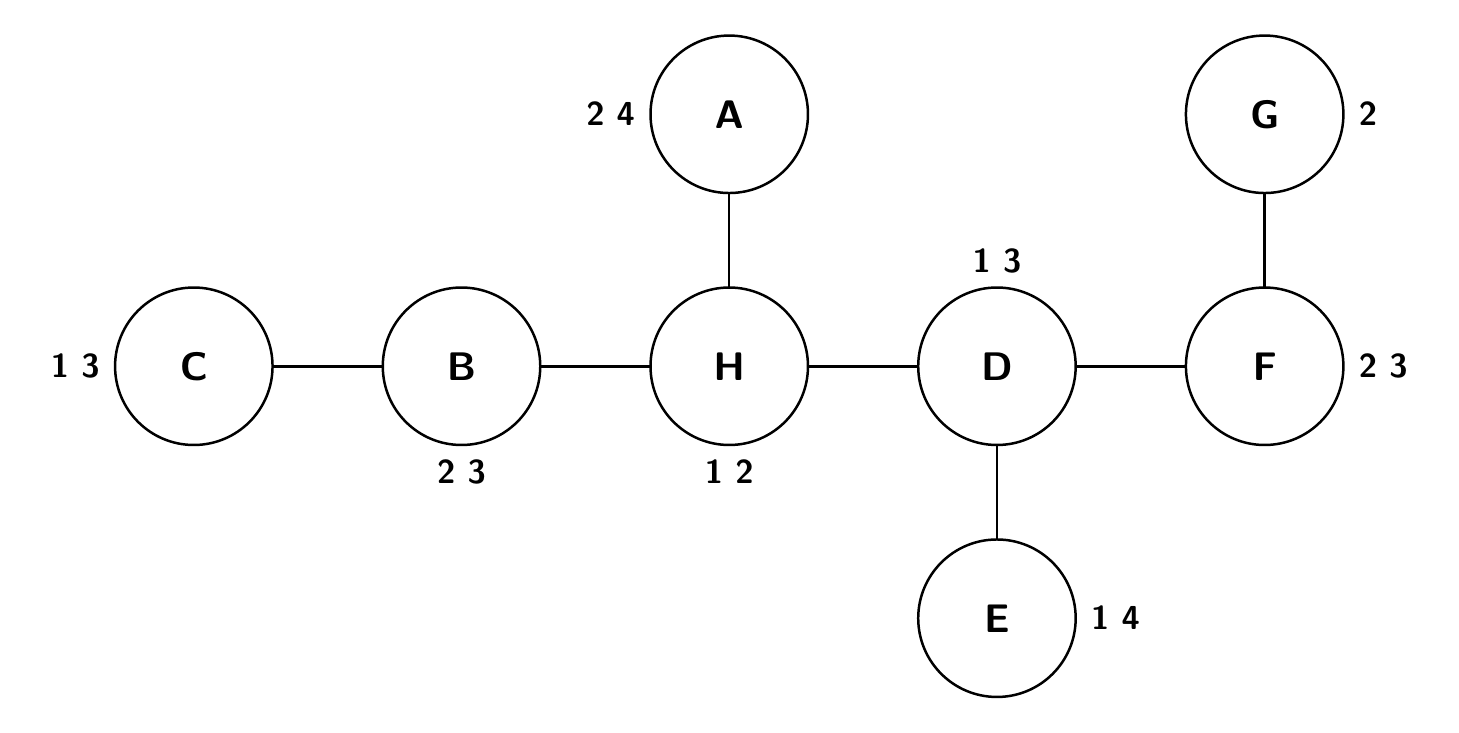
\begin{tikzpicture}[x=1mm, y=1mm]
\useasboundingbox (-89.1,-43.0) rectangle (89.1,43.0);
\draw[line width=0.9pt] (0.00,0.00) -- (0.00,32.00);
\draw[line width=0.9pt] (0.00,0.00) -- (-34.00,0.00);
\draw[line width=0.9pt] (-34.00,0.00) -- (-68.00,0.00);
\draw[line width=0.9pt] (0.00,0.00) -- (34.00,0.00);
\draw[line width=0.9pt] (34.00,0.00) -- (34.00,-32.00);
\draw[line width=0.9pt] (34.00,0.00) -- (68.00,0.00);
\draw[line width=0.9pt] (68.00,0.00) -- (68.00,32.00);
\draw[line width=0.9pt, fill=white] (0.00,32.00) circle (10.0mm);
\node[font=\Large\bfseries] at (0.00,32.00) {A};
\draw[line width=0.9pt, fill=white] (0.00,0.00) circle (10.0mm);
\node[font=\Large\bfseries] at (0.00,0.00) {H};
\draw[line width=0.9pt, fill=white] (-34.00,0.00) circle (10.0mm);
\node[font=\Large\bfseries] at (-34.00,0.00) {B};
\draw[line width=0.9pt, fill=white] (-68.00,0.00) circle (10.0mm);
\node[font=\Large\bfseries] at (-68.00,0.00) {C};
\draw[line width=0.9pt, fill=white] (34.00,0.00) circle (10.0mm);
\node[font=\Large\bfseries] at (34.00,0.00) {D};
\draw[line width=0.9pt, fill=white] (34.00,-32.00) circle (10.0mm);
\node[font=\Large\bfseries] at (34.00,-32.00) {E};
\draw[line width=0.9pt, fill=white] (68.00,0.00) circle (10.0mm);
\node[font=\Large\bfseries] at (68.00,0.00) {F};
\draw[line width=0.9pt, fill=white] (68.00,32.00) circle (10.0mm);
\node[font=\Large\bfseries] at (68.00,32.00) {G};
\node[font=\large\bfseries, inner sep=0.5mm, anchor=90] at (-0.00,-11.40) {1\,\,2};
\node[font=\large\bfseries, inner sep=0.5mm, anchor=0] at (-11.40,32.00) {2\,\,4};
\node[font=\large\bfseries, inner sep=0.5mm, anchor=90] at (-34.00,-11.40) {2\,\,3};
\node[font=\large\bfseries, inner sep=0.5mm, anchor=0] at (-79.40,0.00) {1\,\,3};
\node[font=\large\bfseries, inner sep=0.5mm, anchor=270] at (34.00,11.40) {1\,\,3};
\node[font=\large\bfseries, inner sep=0.5mm, anchor=180] at (45.40,-32.00) {1\,\,4};
\node[font=\large\bfseries, inner sep=0.5mm, anchor=180] at (79.40,0.00) {2\,\,3};
\node[font=\large\bfseries, inner sep=0.5mm, anchor=180] at (79.40,32.00) {2};
\end{tikzpicture}}\par
\vspace{7mm}
\noindent\makebox[\linewidth][c]{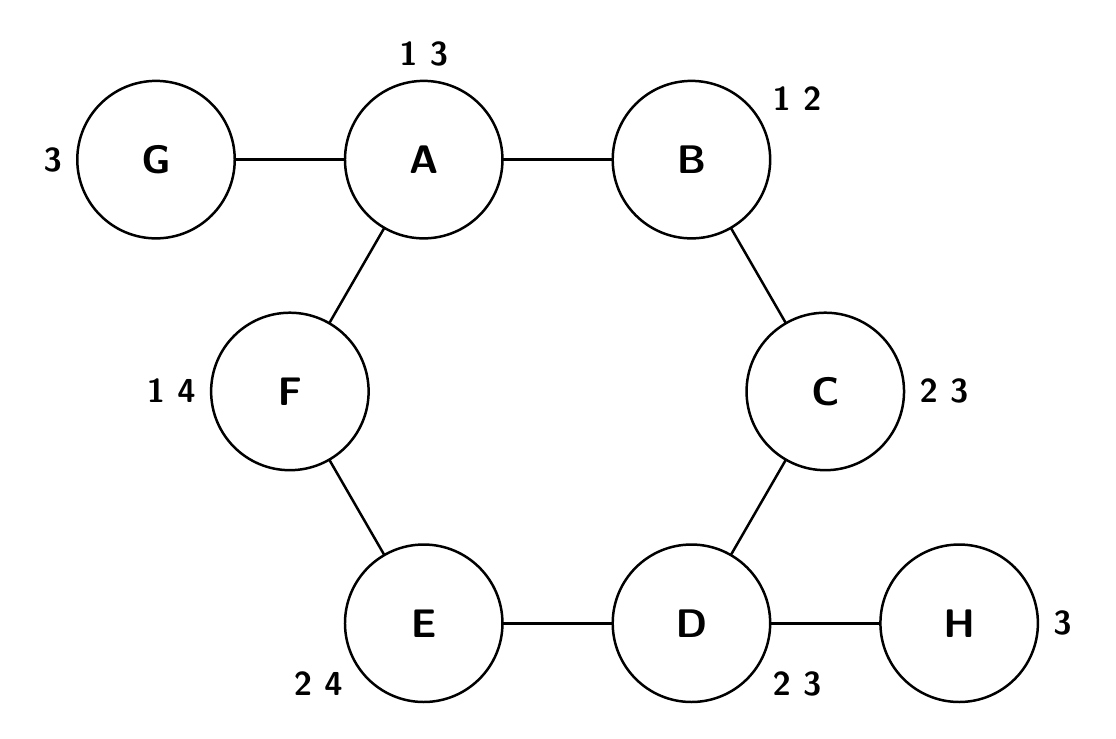
\begin{tikzpicture}[x=1mm, y=1mm]
\useasboundingbox (-67.3,-40.5) rectangle (67.3,46.2);
\draw[line width=0.9pt] (-17.00,29.44) -- (17.00,29.44);
\draw[line width=0.9pt] (17.00,29.44) -- (34.00,0.00);
\draw[line width=0.9pt] (34.00,0.00) -- (17.00,-29.44);
\draw[line width=0.9pt] (17.00,-29.44) -- (-17.00,-29.44);
\draw[line width=0.9pt] (-17.00,-29.44) -- (-34.00,-0.00);
\draw[line width=0.9pt] (-34.00,-0.00) -- (-17.00,29.44);
\draw[line width=0.9pt] (-17.00,29.44) -- (-51.00,29.44);
\draw[line width=0.9pt] (17.00,-29.44) -- (51.00,-29.44);
\draw[line width=0.9pt, fill=white] (-17.00,29.44) circle (10.0mm);
\node[font=\Large\bfseries] at (-17.00,29.44) {A};
\draw[line width=0.9pt, fill=white] (17.00,29.44) circle (10.0mm);
\node[font=\Large\bfseries] at (17.00,29.44) {B};
\draw[line width=0.9pt, fill=white] (34.00,0.00) circle (10.0mm);
\node[font=\Large\bfseries] at (34.00,0.00) {C};
\draw[line width=0.9pt, fill=white] (17.00,-29.44) circle (10.0mm);
\node[font=\Large\bfseries] at (17.00,-29.44) {D};
\draw[line width=0.9pt, fill=white] (-17.00,-29.44) circle (10.0mm);
\node[font=\Large\bfseries] at (-17.00,-29.44) {E};
\draw[line width=0.9pt, fill=white] (-34.00,-0.00) circle (10.0mm);
\node[font=\Large\bfseries] at (-34.00,-0.00) {F};
\draw[line width=0.9pt, fill=white] (-51.00,29.44) circle (10.0mm);
\node[font=\Large\bfseries] at (-51.00,29.44) {G};
\draw[line width=0.9pt, fill=white] (51.00,-29.44) circle (10.0mm);
\node[font=\Large\bfseries] at (51.00,-29.44) {H};
\node[font=\large\bfseries, inner sep=0.5mm, anchor=0] at (-62.40,29.44) {3};
\node[font=\large\bfseries, inner sep=0.5mm, anchor=270] at (-17.00,40.84) {1\,\,3};
\node[font=\large\bfseries, inner sep=0.5mm, anchor=210] at (26.87,35.14) {1\,\,2};
\node[font=\large\bfseries, inner sep=0.5mm, anchor=180] at (45.40,0.00) {2\,\,3};
\node[font=\large\bfseries, inner sep=0.5mm, anchor=150] at (26.87,-35.14) {2\,\,3};
\node[font=\large\bfseries, inner sep=0.5mm, anchor=180] at (62.40,-29.44) {3};
\node[font=\large\bfseries, inner sep=0.5mm, anchor=30] at (-26.87,-35.14) {2\,\,4};
\node[font=\large\bfseries, inner sep=0.5mm, anchor=0] at (-45.40,-0.00) {1\,\,4};
\end{tikzpicture}}\par
\newpage
\textbf{Problem 2:} Which of these can be done?\par
\vspace{8mm}
\noindent\makebox[\linewidth][s]{\hfill 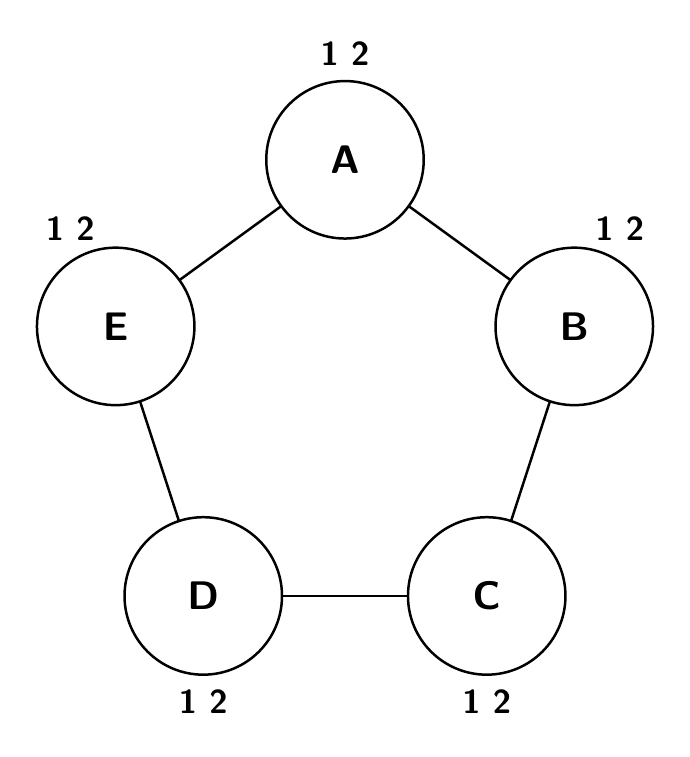
\begin{tikzpicture}[x=1mm, y=1mm]
\useasboundingbox (-40.3,-41.6) rectangle (40.3,47.4);
\draw[line width=0.9pt] (0.00,30.62) -- (29.12,9.46);
\draw[line width=0.9pt] (29.12,9.46) -- (18.00,-24.77);
\draw[line width=0.9pt] (18.00,-24.77) -- (-18.00,-24.77);
\draw[line width=0.9pt] (-18.00,-24.77) -- (-29.12,9.46);
\draw[line width=0.9pt] (-29.12,9.46) -- (0.00,30.62);
\draw[line width=0.9pt, fill=white] (0.00,30.62) circle (10.0mm);
\node[font=\Large\bfseries] at (0.00,30.62) {A};
\draw[line width=0.9pt, fill=white] (29.12,9.46) circle (10.0mm);
\node[font=\Large\bfseries] at (29.12,9.46) {B};
\draw[line width=0.9pt, fill=white] (18.00,-24.77) circle (10.0mm);
\node[font=\Large\bfseries] at (18.00,-24.77) {C};
\draw[line width=0.9pt, fill=white] (-18.00,-24.77) circle (10.0mm);
\node[font=\Large\bfseries] at (-18.00,-24.77) {D};
\draw[line width=0.9pt, fill=white] (-29.12,9.46) circle (10.0mm);
\node[font=\Large\bfseries] at (-29.12,9.46) {E};
\node[font=\large\bfseries, inner sep=0.5mm, anchor=270] at (0.00,42.02) {1\,\,2};
\node[font=\large\bfseries, inner sep=0.5mm, anchor=245] at (33.94,19.80) {1\,\,2};
\node[font=\large\bfseries, inner sep=0.5mm, anchor=90] at (18.00,-36.17) {1\,\,2};
\node[font=\large\bfseries, inner sep=0.5mm, anchor=90] at (-18.00,-36.17) {1\,\,2};
\node[font=\large\bfseries, inner sep=0.5mm, anchor=295] at (-33.94,19.80) {1\,\,2};
\end{tikzpicture} \hfill 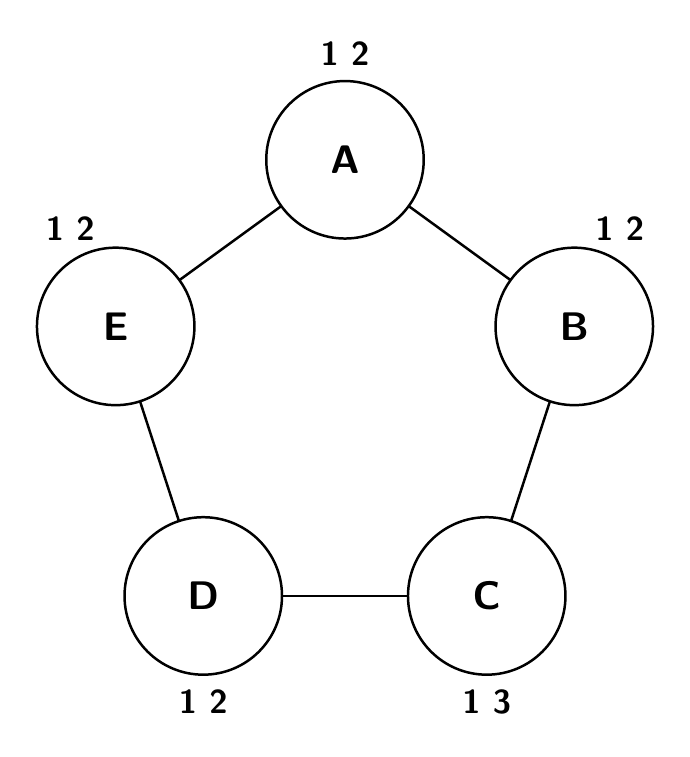
\begin{tikzpicture}[x=1mm, y=1mm]
\useasboundingbox (-40.3,-41.6) rectangle (40.3,47.4);
\draw[line width=0.9pt] (0.00,30.62) -- (29.12,9.46);
\draw[line width=0.9pt] (29.12,9.46) -- (18.00,-24.77);
\draw[line width=0.9pt] (18.00,-24.77) -- (-18.00,-24.77);
\draw[line width=0.9pt] (-18.00,-24.77) -- (-29.12,9.46);
\draw[line width=0.9pt] (-29.12,9.46) -- (0.00,30.62);
\draw[line width=0.9pt, fill=white] (0.00,30.62) circle (10.0mm);
\node[font=\Large\bfseries] at (0.00,30.62) {A};
\draw[line width=0.9pt, fill=white] (29.12,9.46) circle (10.0mm);
\node[font=\Large\bfseries] at (29.12,9.46) {B};
\draw[line width=0.9pt, fill=white] (18.00,-24.77) circle (10.0mm);
\node[font=\Large\bfseries] at (18.00,-24.77) {C};
\draw[line width=0.9pt, fill=white] (-18.00,-24.77) circle (10.0mm);
\node[font=\Large\bfseries] at (-18.00,-24.77) {D};
\draw[line width=0.9pt, fill=white] (-29.12,9.46) circle (10.0mm);
\node[font=\Large\bfseries] at (-29.12,9.46) {E};
\node[font=\large\bfseries, inner sep=0.5mm, anchor=270] at (0.00,42.02) {1\,\,2};
\node[font=\large\bfseries, inner sep=0.5mm, anchor=245] at (33.94,19.80) {1\,\,2};
\node[font=\large\bfseries, inner sep=0.5mm, anchor=90] at (18.00,-36.17) {1\,\,3};
\node[font=\large\bfseries, inner sep=0.5mm, anchor=90] at (-18.00,-36.17) {1\,\,2};
\node[font=\large\bfseries, inner sep=0.5mm, anchor=295] at (-33.94,19.80) {1\,\,2};
\end{tikzpicture} \hfill}\par
\vspace{12mm}
\noindent\makebox[\linewidth][s]{\hfill 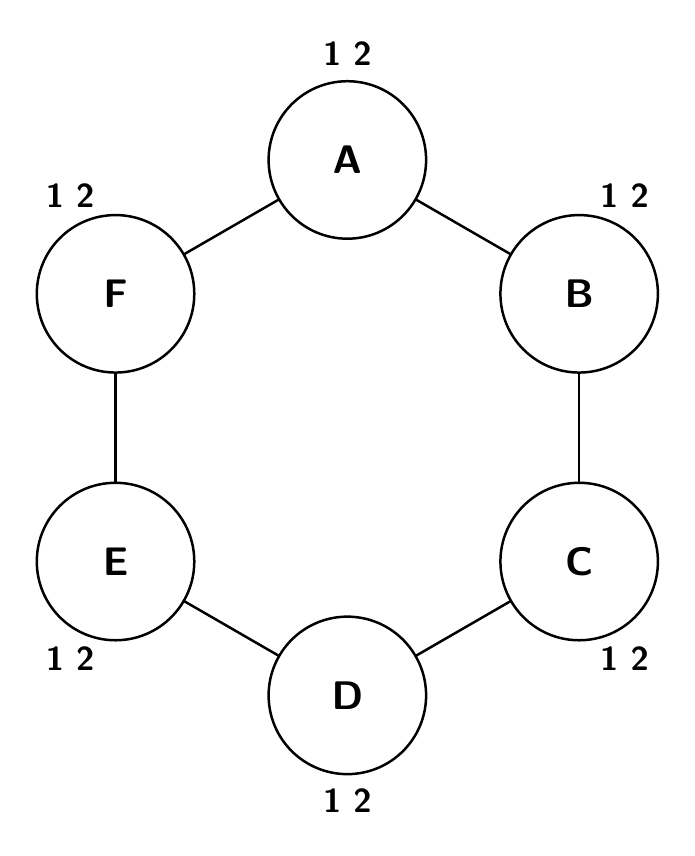
\begin{tikzpicture}[x=1mm, y=1mm]
\useasboundingbox (-40.6,-50.8) rectangle (40.6,50.8);
\draw[line width=0.9pt] (0.00,34.00) -- (29.44,17.00);
\draw[line width=0.9pt] (29.44,17.00) -- (29.44,-17.00);
\draw[line width=0.9pt] (29.44,-17.00) -- (0.00,-34.00);
\draw[line width=0.9pt] (0.00,-34.00) -- (-29.44,-17.00);
\draw[line width=0.9pt] (-29.44,-17.00) -- (-29.44,17.00);
\draw[line width=0.9pt] (-29.44,17.00) -- (0.00,34.00);
\draw[line width=0.9pt, fill=white] (0.00,34.00) circle (10.0mm);
\node[font=\Large\bfseries] at (0.00,34.00) {A};
\draw[line width=0.9pt, fill=white] (29.44,17.00) circle (10.0mm);
\node[font=\Large\bfseries] at (29.44,17.00) {B};
\draw[line width=0.9pt, fill=white] (29.44,-17.00) circle (10.0mm);
\node[font=\Large\bfseries] at (29.44,-17.00) {C};
\draw[line width=0.9pt, fill=white] (0.00,-34.00) circle (10.0mm);
\node[font=\Large\bfseries] at (0.00,-34.00) {D};
\draw[line width=0.9pt, fill=white] (-29.44,-17.00) circle (10.0mm);
\node[font=\Large\bfseries] at (-29.44,-17.00) {E};
\draw[line width=0.9pt, fill=white] (-29.44,17.00) circle (10.0mm);
\node[font=\Large\bfseries] at (-29.44,17.00) {F};
\node[font=\large\bfseries, inner sep=0.5mm, anchor=270] at (0.00,45.40) {1\,\,2};
\node[font=\large\bfseries, inner sep=0.5mm, anchor=245] at (34.26,27.33) {1\,\,2};
\node[font=\large\bfseries, inner sep=0.5mm, anchor=115] at (34.26,-27.33) {1\,\,2};
\node[font=\large\bfseries, inner sep=0.5mm, anchor=90] at (-0.00,-45.40) {1\,\,2};
\node[font=\large\bfseries, inner sep=0.5mm, anchor=65] at (-34.26,-27.33) {1\,\,2};
\node[font=\large\bfseries, inner sep=0.5mm, anchor=295] at (-34.26,27.33) {1\,\,2};
\end{tikzpicture} \hfill 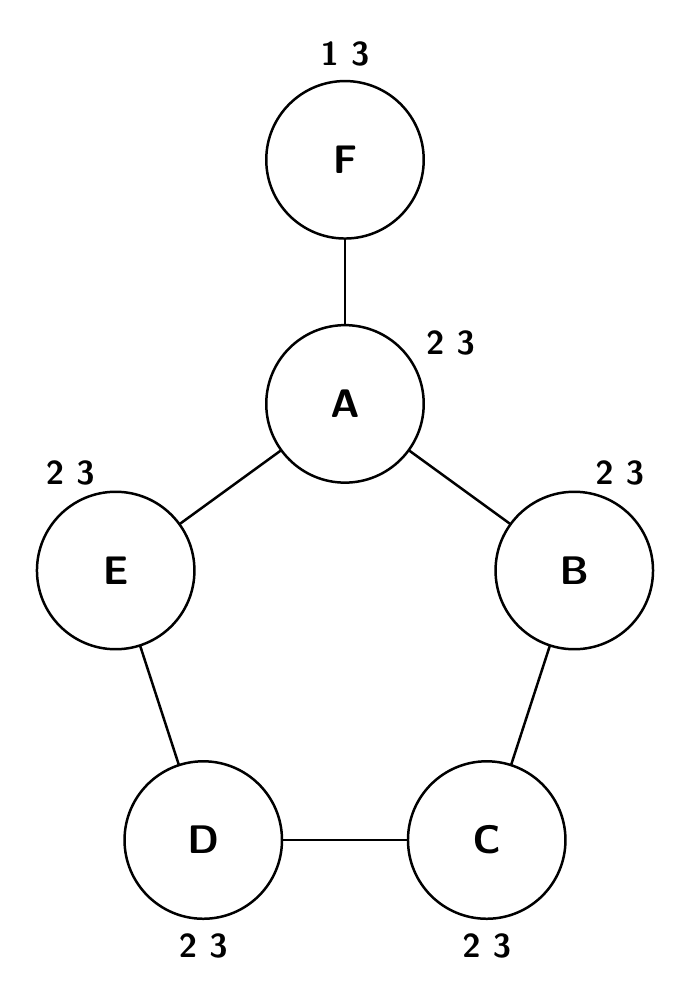
\begin{tikzpicture}[x=1mm, y=1mm]
\useasboundingbox (-40.3,-41.6) rectangle (40.3,78.4);
\draw[line width=0.9pt] (0.00,30.62) -- (29.12,9.46);
\draw[line width=0.9pt] (29.12,9.46) -- (18.00,-24.77);
\draw[line width=0.9pt] (18.00,-24.77) -- (-18.00,-24.77);
\draw[line width=0.9pt] (-18.00,-24.77) -- (-29.12,9.46);
\draw[line width=0.9pt] (-29.12,9.46) -- (0.00,30.62);
\draw[line width=0.9pt] (0.00,30.62) -- (0.00,61.62);
\draw[line width=0.9pt, fill=white] (0.00,30.62) circle (10.0mm);
\node[font=\Large\bfseries] at (0.00,30.62) {A};
\draw[line width=0.9pt, fill=white] (29.12,9.46) circle (10.0mm);
\node[font=\Large\bfseries] at (29.12,9.46) {B};
\draw[line width=0.9pt, fill=white] (18.00,-24.77) circle (10.0mm);
\node[font=\Large\bfseries] at (18.00,-24.77) {C};
\draw[line width=0.9pt, fill=white] (-18.00,-24.77) circle (10.0mm);
\node[font=\Large\bfseries] at (-18.00,-24.77) {D};
\draw[line width=0.9pt, fill=white] (-29.12,9.46) circle (10.0mm);
\node[font=\Large\bfseries] at (-29.12,9.46) {E};
\draw[line width=0.9pt, fill=white] (0.00,61.62) circle (10.0mm);
\node[font=\Large\bfseries] at (0.00,61.62) {F};
\node[font=\large\bfseries, inner sep=0.5mm, anchor=210] at (9.87,36.32) {2\,\,3};
\node[font=\large\bfseries, inner sep=0.5mm, anchor=245] at (33.94,19.80) {2\,\,3};
\node[font=\large\bfseries, inner sep=0.5mm, anchor=90] at (18.00,-36.17) {2\,\,3};
\node[font=\large\bfseries, inner sep=0.5mm, anchor=90] at (-18.00,-36.17) {2\,\,3};
\node[font=\large\bfseries, inner sep=0.5mm, anchor=295] at (-33.94,19.80) {2\,\,3};
\node[font=\large\bfseries, inner sep=0.5mm, anchor=270] at (0.00,73.02) {1\,\,3};
\end{tikzpicture} \hfill}\par
\newpage
\textbf{Problem 3:} Which of these can be done?\par
\vspace{12mm}
\noindent\makebox[\linewidth][c]{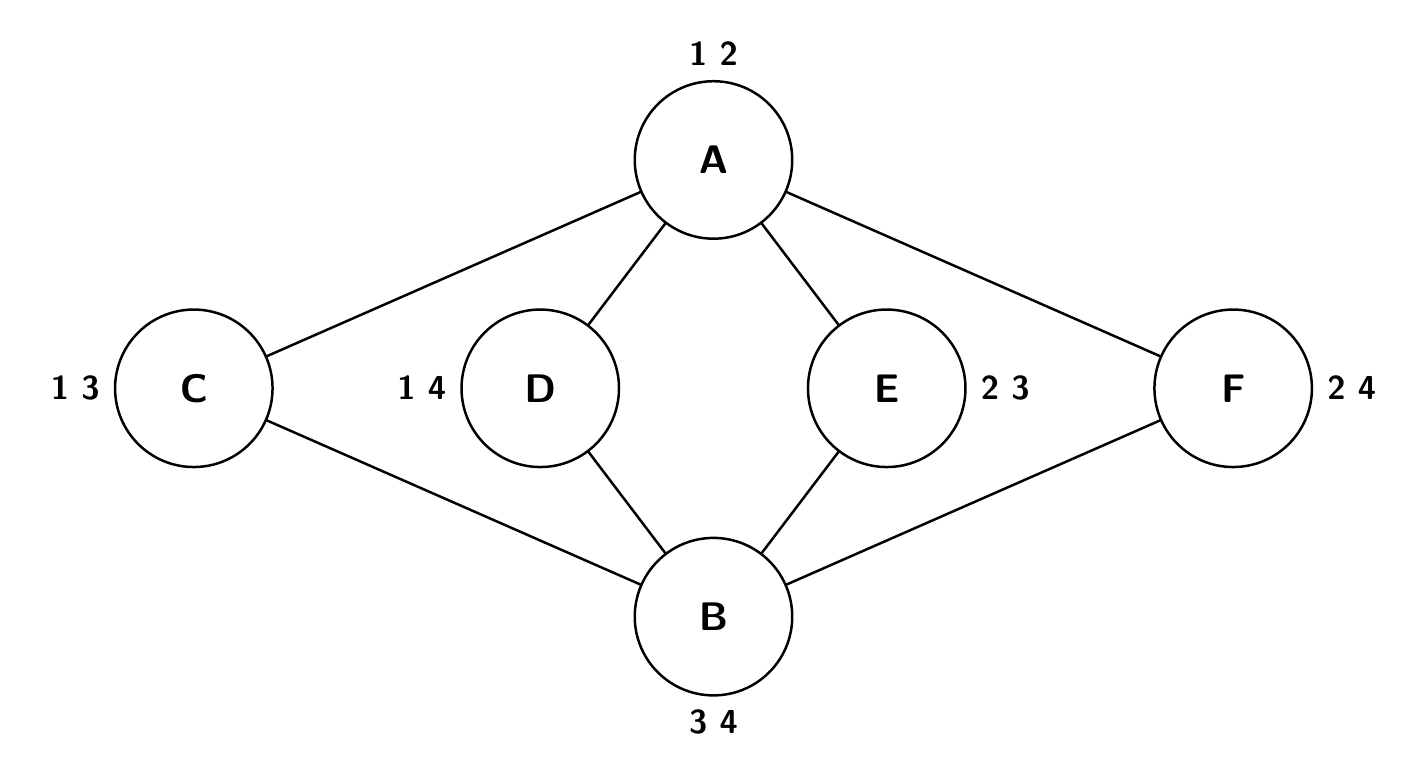
\begin{tikzpicture}[x=1mm, y=1mm]
\useasboundingbox (-87.1,-45.8) rectangle (87.1,45.8);
\draw[line width=0.9pt] (0.00,29.00) -- (-66.00,0.00);
\draw[line width=0.9pt] (0.00,29.00) -- (-22.00,0.00);
\draw[line width=0.9pt] (0.00,29.00) -- (22.00,0.00);
\draw[line width=0.9pt] (0.00,29.00) -- (66.00,0.00);
\draw[line width=0.9pt] (0.00,-29.00) -- (-66.00,0.00);
\draw[line width=0.9pt] (0.00,-29.00) -- (-22.00,0.00);
\draw[line width=0.9pt] (0.00,-29.00) -- (22.00,0.00);
\draw[line width=0.9pt] (0.00,-29.00) -- (66.00,0.00);
\draw[line width=0.9pt, fill=white] (0.00,29.00) circle (10.0mm);
\node[font=\Large\bfseries] at (0.00,29.00) {A};
\draw[line width=0.9pt, fill=white] (0.00,-29.00) circle (10.0mm);
\node[font=\Large\bfseries] at (0.00,-29.00) {B};
\draw[line width=0.9pt, fill=white] (-66.00,0.00) circle (10.0mm);
\node[font=\Large\bfseries] at (-66.00,0.00) {C};
\draw[line width=0.9pt, fill=white] (-22.00,0.00) circle (10.0mm);
\node[font=\Large\bfseries] at (-22.00,0.00) {D};
\draw[line width=0.9pt, fill=white] (22.00,0.00) circle (10.0mm);
\node[font=\Large\bfseries] at (22.00,0.00) {E};
\draw[line width=0.9pt, fill=white] (66.00,0.00) circle (10.0mm);
\node[font=\Large\bfseries] at (66.00,0.00) {F};
\node[font=\large\bfseries, inner sep=0.5mm, anchor=270] at (0.00,40.40) {1\,\,2};
\node[font=\large\bfseries, inner sep=0.5mm, anchor=90] at (-0.00,-40.40) {3\,\,4};
\node[font=\large\bfseries, inner sep=0.5mm, anchor=0] at (-77.40,0.00) {1\,\,3};
\node[font=\large\bfseries, inner sep=0.5mm, anchor=0] at (-33.40,0.00) {1\,\,4};
\node[font=\large\bfseries, inner sep=0.5mm, anchor=180] at (33.40,0.00) {2\,\,3};
\node[font=\large\bfseries, inner sep=0.5mm, anchor=180] at (77.40,0.00) {2\,\,4};
\end{tikzpicture}}\par
\vspace{22mm}
\noindent\makebox[\linewidth][c]{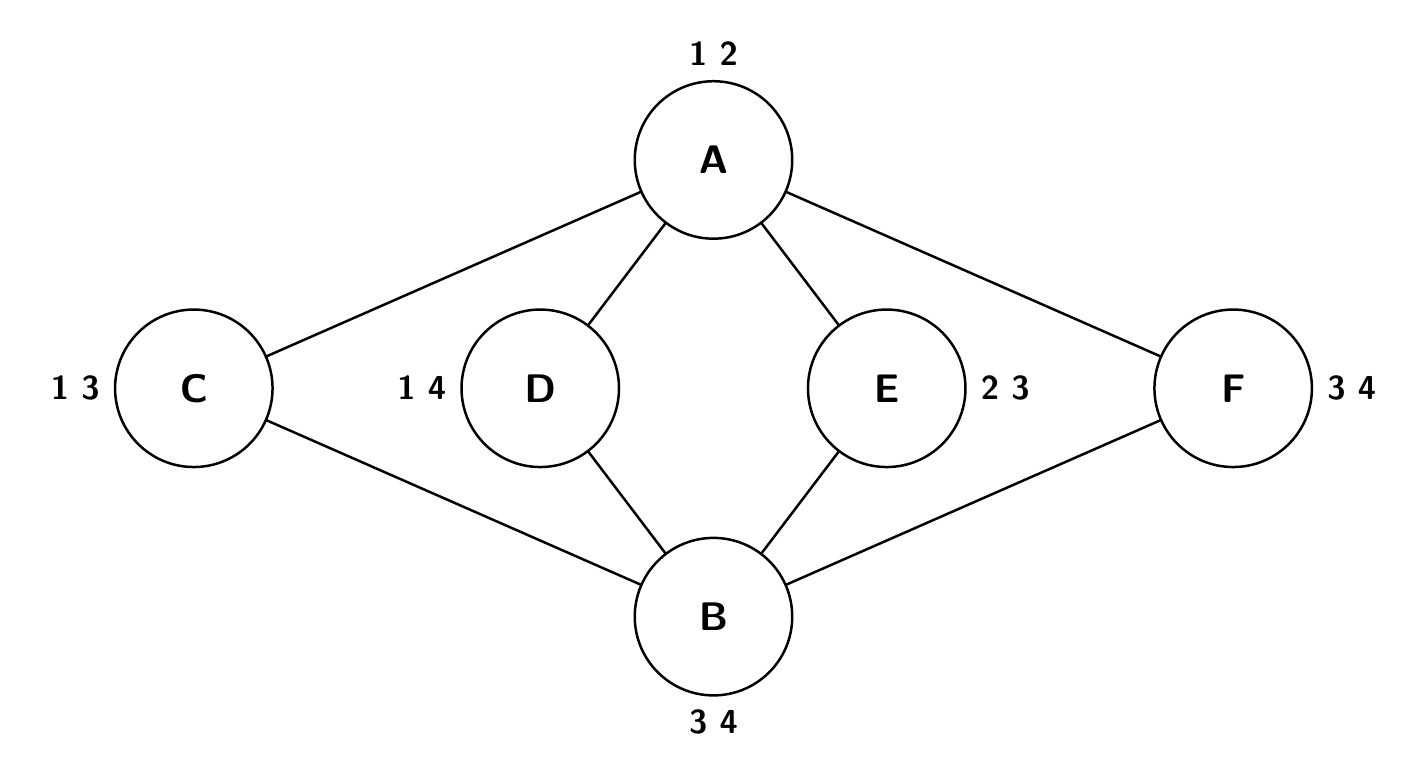
\begin{tikzpicture}[x=1mm, y=1mm]
\useasboundingbox (-87.1,-45.8) rectangle (87.1,45.8);
\draw[line width=0.9pt] (0.00,29.00) -- (-66.00,0.00);
\draw[line width=0.9pt] (0.00,29.00) -- (-22.00,0.00);
\draw[line width=0.9pt] (0.00,29.00) -- (22.00,0.00);
\draw[line width=0.9pt] (0.00,29.00) -- (66.00,0.00);
\draw[line width=0.9pt] (0.00,-29.00) -- (-66.00,0.00);
\draw[line width=0.9pt] (0.00,-29.00) -- (-22.00,0.00);
\draw[line width=0.9pt] (0.00,-29.00) -- (22.00,0.00);
\draw[line width=0.9pt] (0.00,-29.00) -- (66.00,0.00);
\draw[line width=0.9pt, fill=white] (0.00,29.00) circle (10.0mm);
\node[font=\Large\bfseries] at (0.00,29.00) {A};
\draw[line width=0.9pt, fill=white] (0.00,-29.00) circle (10.0mm);
\node[font=\Large\bfseries] at (0.00,-29.00) {B};
\draw[line width=0.9pt, fill=white] (-66.00,0.00) circle (10.0mm);
\node[font=\Large\bfseries] at (-66.00,0.00) {C};
\draw[line width=0.9pt, fill=white] (-22.00,0.00) circle (10.0mm);
\node[font=\Large\bfseries] at (-22.00,0.00) {D};
\draw[line width=0.9pt, fill=white] (22.00,0.00) circle (10.0mm);
\node[font=\Large\bfseries] at (22.00,0.00) {E};
\draw[line width=0.9pt, fill=white] (66.00,0.00) circle (10.0mm);
\node[font=\Large\bfseries] at (66.00,0.00) {F};
\node[font=\large\bfseries, inner sep=0.5mm, anchor=270] at (0.00,40.40) {1\,\,2};
\node[font=\large\bfseries, inner sep=0.5mm, anchor=90] at (-0.00,-40.40) {3\,\,4};
\node[font=\large\bfseries, inner sep=0.5mm, anchor=0] at (-77.40,0.00) {1\,\,3};
\node[font=\large\bfseries, inner sep=0.5mm, anchor=0] at (-33.40,0.00) {1\,\,4};
\node[font=\large\bfseries, inner sep=0.5mm, anchor=180] at (33.40,0.00) {2\,\,3};
\node[font=\large\bfseries, inner sep=0.5mm, anchor=180] at (77.40,0.00) {3\,\,4};
\end{tikzpicture}}\par
\newpage
\textbf{Problem 4:} For each network, can you write two of the numbers 1, 2, 3, 4 next to every circle without numbers, so that it can't be done?\par
\vspace{6mm}
\noindent\makebox[\linewidth][c]{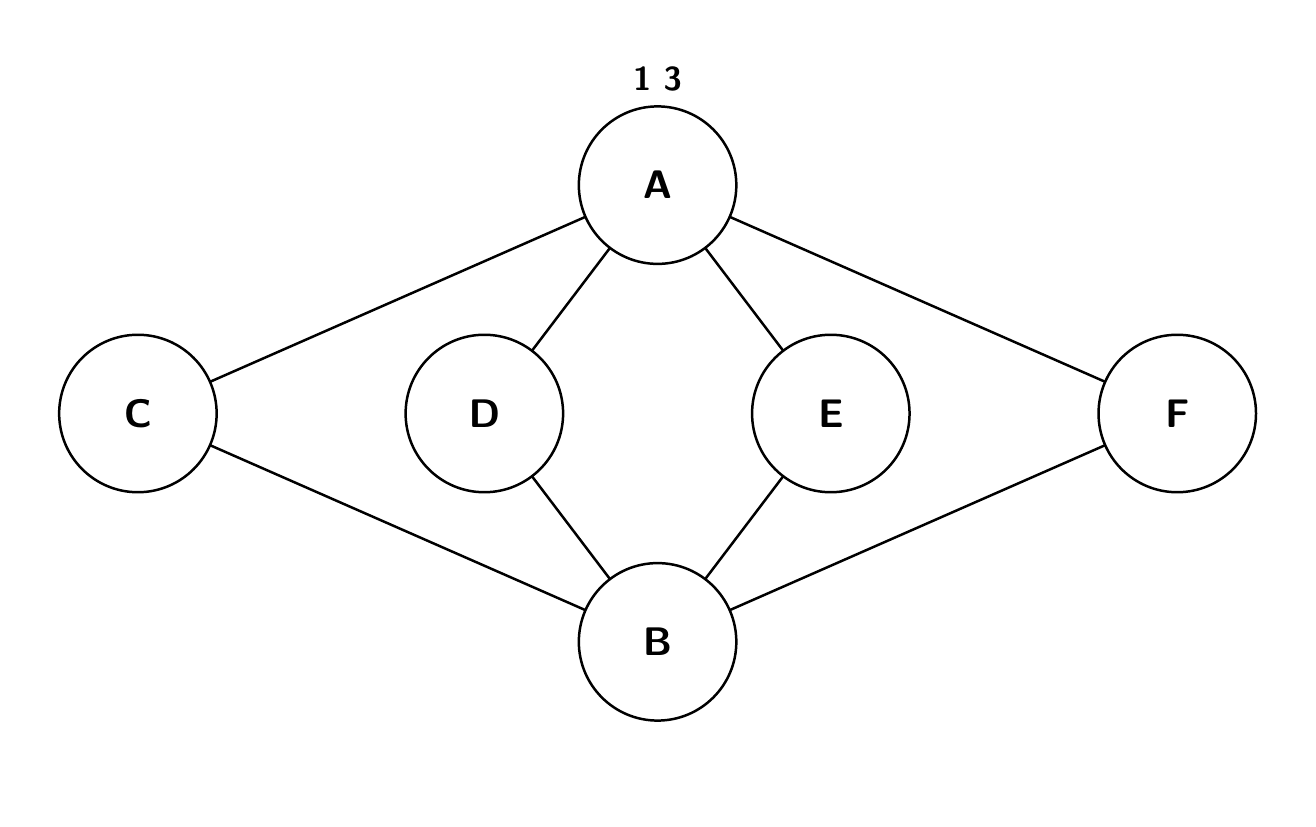
\begin{tikzpicture}[x=1mm, y=1mm]
\useasboundingbox (-80.0,-49.0) rectangle (80.0,49.0);
\draw[line width=0.9pt] (0.00,29.00) -- (-66.00,0.00);
\draw[line width=0.9pt] (0.00,29.00) -- (-22.00,0.00);
\draw[line width=0.9pt] (0.00,29.00) -- (22.00,0.00);
\draw[line width=0.9pt] (0.00,29.00) -- (66.00,0.00);
\draw[line width=0.9pt] (0.00,-29.00) -- (-66.00,0.00);
\draw[line width=0.9pt] (0.00,-29.00) -- (-22.00,0.00);
\draw[line width=0.9pt] (0.00,-29.00) -- (22.00,0.00);
\draw[line width=0.9pt] (0.00,-29.00) -- (66.00,0.00);
\draw[line width=0.9pt, fill=white] (0.00,29.00) circle (10.0mm);
\node[font=\Large\bfseries] at (0.00,29.00) {A};
\draw[line width=0.9pt, fill=white] (0.00,-29.00) circle (10.0mm);
\node[font=\Large\bfseries] at (0.00,-29.00) {B};
\draw[line width=0.9pt, fill=white] (-66.00,0.00) circle (10.0mm);
\node[font=\Large\bfseries] at (-66.00,0.00) {C};
\draw[line width=0.9pt, fill=white] (-22.00,0.00) circle (10.0mm);
\node[font=\Large\bfseries] at (-22.00,0.00) {D};
\draw[line width=0.9pt, fill=white] (22.00,0.00) circle (10.0mm);
\node[font=\Large\bfseries] at (22.00,0.00) {E};
\draw[line width=0.9pt, fill=white] (66.00,0.00) circle (10.0mm);
\node[font=\Large\bfseries] at (66.00,0.00) {F};
\node[font=\large\bfseries, inner sep=0.5mm, anchor=270] at (0.00,40.40) {1\,\,3};
\end{tikzpicture}}\par
\vspace{12mm}
\noindent\makebox[\linewidth][c]{\begin{tikzpicture}[x=1mm, y=1mm]
\useasboundingbox (-62.0,-52.0) rectangle (62.0,52.0);
\draw[line width=0.9pt] (0.00,32.00) -- (-38.00,0.00);
\draw[line width=0.9pt] (0.00,32.00) -- (0.00,0.00);
\draw[line width=0.9pt] (0.00,32.00) -- (38.00,0.00);
\draw[line width=0.9pt] (0.00,-32.00) -- (-38.00,0.00);
\draw[line width=0.9pt] (0.00,-32.00) -- (0.00,0.00);
\draw[line width=0.9pt] (0.00,-32.00) -- (38.00,0.00);
\draw[line width=0.9pt, fill=white] (0.00,32.00) circle (10.0mm);
\node[font=\Large\bfseries] at (0.00,32.00) {A};
\draw[line width=0.9pt, fill=white] (0.00,-32.00) circle (10.0mm);
\node[font=\Large\bfseries] at (0.00,-32.00) {B};
\draw[line width=0.9pt, fill=white] (-38.00,0.00) circle (10.0mm);
\node[font=\Large\bfseries] at (-38.00,0.00) {C};
\draw[line width=0.9pt, fill=white] (0.00,0.00) circle (10.0mm);
\node[font=\Large\bfseries] at (0.00,0.00) {D};
\draw[line width=0.9pt, fill=white] (38.00,0.00) circle (10.0mm);
\node[font=\Large\bfseries] at (38.00,0.00) {E};
\node[font=\large\bfseries, inner sep=0.5mm, anchor=270] at (0.00,43.40) {1\,\,3};
\end{tikzpicture}}\par
\newpage
A move takes one counter off a circle and puts a counter with a different number there. After every move, no line may have the same number at both ends. Write a move as the circle's letter and its new number, like D1.\par
\vspace{3mm}
\noindent\makebox[\linewidth][c]{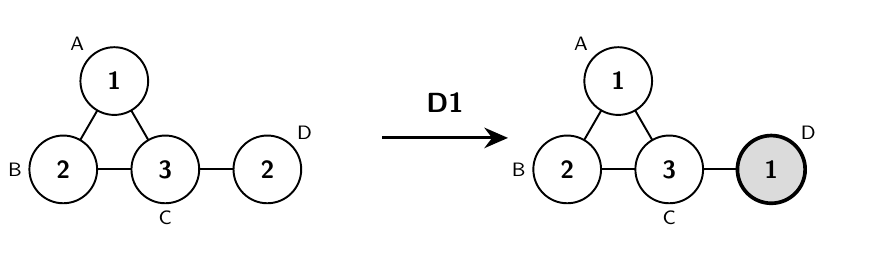
\begin{tikzpicture}[x=1mm, y=1mm]
\useasboundingbox (-11.0,-7.0) rectangle (95.0,18.0);
\draw[line width=0.7pt] (0.00,11.22) -- (-6.48,0.00);
\draw[line width=0.7pt] (-6.48,0.00) -- (6.48,0.00);
\draw[line width=0.7pt] (6.48,0.00) -- (0.00,11.22);
\draw[line width=0.7pt] (6.48,0.00) -- (19.44,0.00);
\draw[line width=0.7pt, fill=white] (0.00,11.22) circle (4.3mm);
\node[font=\small\bfseries] at (0.00,11.22) {1};
\node[font=\scriptsize, inner sep=0.4mm, anchor=315] at (-3.39,14.62) {A};
\draw[line width=0.7pt, fill=white] (-6.48,0.00) circle (4.3mm);
\node[font=\small\bfseries] at (-6.48,0.00) {2};
\node[font=\scriptsize, inner sep=0.4mm, anchor=0] at (-11.28,0.00) {B};
\draw[line width=0.7pt, fill=white] (6.48,0.00) circle (4.3mm);
\node[font=\small\bfseries] at (6.48,0.00) {3};
\node[font=\scriptsize, inner sep=0.4mm, anchor=90] at (6.48,-4.80) {C};
\draw[line width=0.7pt, fill=white] (19.44,0.00) circle (4.3mm);
\node[font=\small\bfseries] at (19.44,0.00) {2};
\node[font=\scriptsize, inner sep=0.4mm, anchor=225] at (22.83,3.39) {D};
\draw[bigarrow] (34.0,4) -- (50.0,4);
\node[font=\bfseries] at (42.0,8.5) {D1};
\draw[line width=0.7pt] (64.00,11.22) -- (57.52,0.00);
\draw[line width=0.7pt] (57.52,0.00) -- (70.48,0.00);
\draw[line width=0.7pt] (70.48,0.00) -- (64.00,11.22);
\draw[line width=0.7pt] (70.48,0.00) -- (83.44,0.00);
\draw[line width=0.7pt, fill=white] (64.00,11.22) circle (4.3mm);
\node[font=\small\bfseries] at (64.00,11.22) {1};
\node[font=\scriptsize, inner sep=0.4mm, anchor=315] at (60.61,14.62) {A};
\draw[line width=0.7pt, fill=white] (57.52,0.00) circle (4.3mm);
\node[font=\small\bfseries] at (57.52,0.00) {2};
\node[font=\scriptsize, inner sep=0.4mm, anchor=0] at (52.72,0.00) {B};
\draw[line width=0.7pt, fill=white] (70.48,0.00) circle (4.3mm);
\node[font=\small\bfseries] at (70.48,0.00) {3};
\node[font=\scriptsize, inner sep=0.4mm, anchor=90] at (70.48,-4.80) {C};
\draw[line width=1.3299999999999998pt, fill=black!14] (83.44,0.00) circle (4.3mm);
\node[font=\small\bfseries] at (83.44,0.00) {1};
\node[font=\scriptsize, inner sep=0.4mm, anchor=225] at (86.83,3.39) {D};
\end{tikzpicture}}\par
\vspace{3mm}
\textbf{Problem 5:} Use counters 1, 2 and 3. Set up Start, then change it into Goal in as few moves as you can. Write your moves.\par
\vspace{8mm}
\noindent\makebox[\linewidth][c]{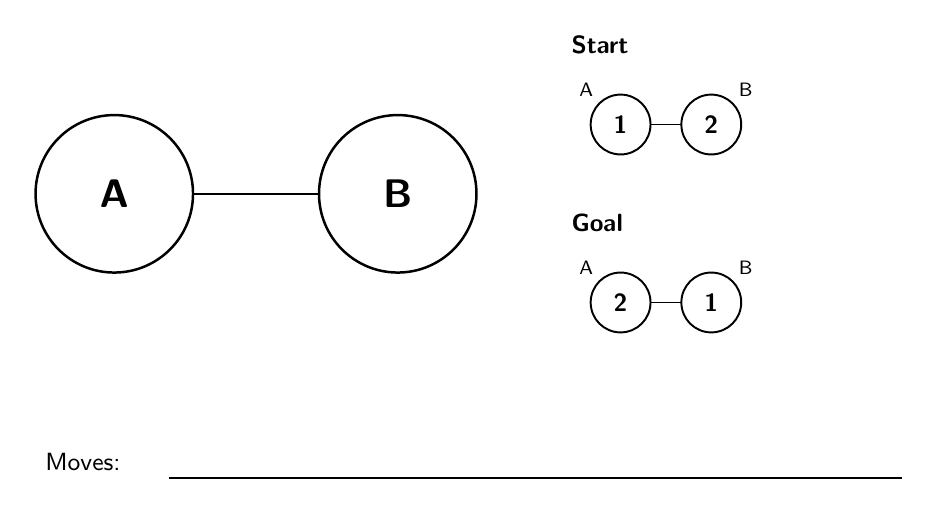
\begin{tikzpicture}[x=1mm, y=1mm]
\useasboundingbox (-11.0,-38.1) rectangle (101.0,21.1);
\draw[line width=0.9pt] (0.00,0.00) -- (36.00,0.00);
\draw[line width=0.9pt, fill=white] (0.00,0.00) circle (10.0mm);
\node[font=\Large\bfseries] at (0.00,0.00) {A};
\draw[line width=0.9pt, fill=white] (36.00,0.00) circle (10.0mm);
\node[font=\Large\bfseries] at (36.00,0.00) {B};
\node[anchor=north west, font=\small\bfseries, inner sep=0] at (58.0,20.1) {Start};
\draw[line width=0.7pt] (64.30,8.80) -- (75.82,8.80);
\draw[line width=0.7pt, fill=white] (64.30,8.80) circle (3.8mm);
\node[font=\small\bfseries] at (64.30,8.80) {1};
\node[font=\scriptsize, inner sep=0.4mm, anchor=315] at (61.26,11.84) {A};
\draw[line width=0.7pt, fill=white] (75.82,8.80) circle (3.8mm);
\node[font=\small\bfseries] at (75.82,8.80) {2};
\node[font=\scriptsize, inner sep=0.4mm, anchor=225] at (78.86,11.84) {B};
\node[anchor=north west, font=\small\bfseries, inner sep=0] at (58.0,-2.5) {Goal};
\draw[line width=0.7pt] (64.30,-13.80) -- (75.82,-13.80);
\draw[line width=0.7pt, fill=white] (64.30,-13.80) circle (3.8mm);
\node[font=\small\bfseries] at (64.30,-13.80) {2};
\node[font=\scriptsize, inner sep=0.4mm, anchor=315] at (61.26,-10.76) {A};
\draw[line width=0.7pt, fill=white] (75.82,-13.80) circle (3.8mm);
\node[font=\small\bfseries] at (75.82,-13.80) {1};
\node[font=\scriptsize, inner sep=0.4mm, anchor=225] at (78.86,-10.76) {B};
\node[anchor=west, font=\small] at (-10.0,-34.1) {Moves:};
\draw[line width=0.5pt] (7.0,-36.1) -- (100.0,-36.1);
\end{tikzpicture}}\par
\vspace{14mm}
\noindent\makebox[\linewidth][c]{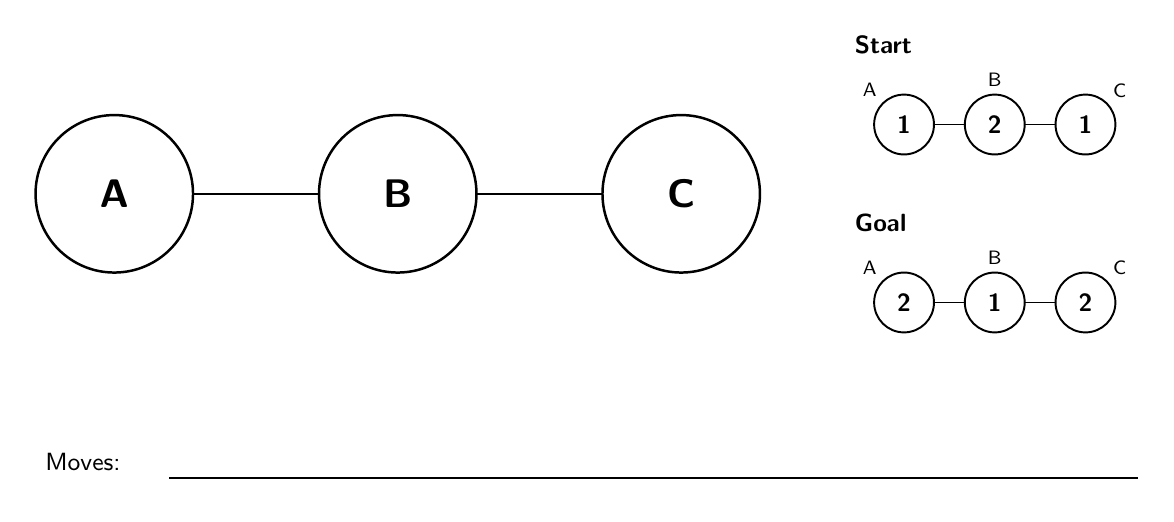
\begin{tikzpicture}[x=1mm, y=1mm]
\useasboundingbox (-11.0,-38.1) rectangle (131.0,21.1);
\draw[line width=0.9pt] (0.00,0.00) -- (36.00,0.00);
\draw[line width=0.9pt] (36.00,0.00) -- (72.00,0.00);
\draw[line width=0.9pt, fill=white] (0.00,0.00) circle (10.0mm);
\node[font=\Large\bfseries] at (0.00,0.00) {A};
\draw[line width=0.9pt, fill=white] (36.00,0.00) circle (10.0mm);
\node[font=\Large\bfseries] at (36.00,0.00) {B};
\draw[line width=0.9pt, fill=white] (72.00,0.00) circle (10.0mm);
\node[font=\Large\bfseries] at (72.00,0.00) {C};
\node[anchor=north west, font=\small\bfseries, inner sep=0] at (94.0,20.1) {Start};
\draw[line width=0.7pt] (100.30,8.80) -- (111.82,8.80);
\draw[line width=0.7pt] (111.82,8.80) -- (123.34,8.80);
\draw[line width=0.7pt, fill=white] (100.30,8.80) circle (3.8mm);
\node[font=\small\bfseries] at (100.30,8.80) {1};
\node[font=\scriptsize, inner sep=0.4mm, anchor=315] at (97.26,11.84) {A};
\draw[line width=0.7pt, fill=white] (111.82,8.80) circle (3.8mm);
\node[font=\small\bfseries] at (111.82,8.80) {2};
\node[font=\scriptsize, inner sep=0.4mm, anchor=270] at (111.82,13.10) {B};
\draw[line width=0.7pt, fill=white] (123.34,8.80) circle (3.8mm);
\node[font=\small\bfseries] at (123.34,8.80) {1};
\node[font=\scriptsize, inner sep=0.4mm, anchor=225] at (126.38,11.84) {C};
\node[anchor=north west, font=\small\bfseries, inner sep=0] at (94.0,-2.5) {Goal};
\draw[line width=0.7pt] (100.30,-13.80) -- (111.82,-13.80);
\draw[line width=0.7pt] (111.82,-13.80) -- (123.34,-13.80);
\draw[line width=0.7pt, fill=white] (100.30,-13.80) circle (3.8mm);
\node[font=\small\bfseries] at (100.30,-13.80) {2};
\node[font=\scriptsize, inner sep=0.4mm, anchor=315] at (97.26,-10.76) {A};
\draw[line width=0.7pt, fill=white] (111.82,-13.80) circle (3.8mm);
\node[font=\small\bfseries] at (111.82,-13.80) {1};
\node[font=\scriptsize, inner sep=0.4mm, anchor=270] at (111.82,-9.50) {B};
\draw[line width=0.7pt, fill=white] (123.34,-13.80) circle (3.8mm);
\node[font=\small\bfseries] at (123.34,-13.80) {2};
\node[font=\scriptsize, inner sep=0.4mm, anchor=225] at (126.38,-10.76) {C};
\node[anchor=west, font=\small] at (-10.0,-34.1) {Moves:};
\draw[line width=0.5pt] (7.0,-36.1) -- (130.0,-36.1);
\end{tikzpicture}}\par
\newpage
\textbf{Problem 6:} Use counters 1, 2 and 3. Change each Start into its Goal in as few moves as you can. Write your moves.\par
\vspace{8mm}
\noindent\makebox[\linewidth][c]{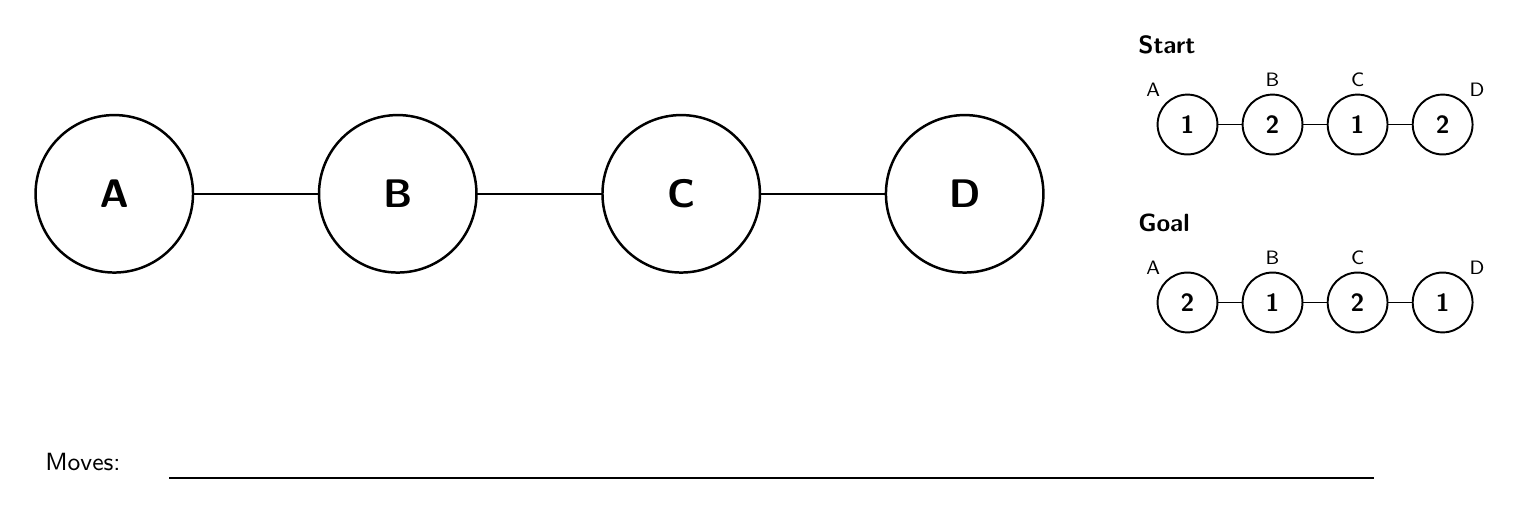
\begin{tikzpicture}[x=1mm, y=1mm]
\useasboundingbox (-11.0,-38.1) rectangle (176.0,21.1);
\draw[line width=0.9pt] (0.00,0.00) -- (36.00,0.00);
\draw[line width=0.9pt] (36.00,0.00) -- (72.00,0.00);
\draw[line width=0.9pt] (72.00,0.00) -- (108.00,0.00);
\draw[line width=0.9pt, fill=white] (0.00,0.00) circle (10.0mm);
\node[font=\Large\bfseries] at (0.00,0.00) {A};
\draw[line width=0.9pt, fill=white] (36.00,0.00) circle (10.0mm);
\node[font=\Large\bfseries] at (36.00,0.00) {B};
\draw[line width=0.9pt, fill=white] (72.00,0.00) circle (10.0mm);
\node[font=\Large\bfseries] at (72.00,0.00) {C};
\draw[line width=0.9pt, fill=white] (108.00,0.00) circle (10.0mm);
\node[font=\Large\bfseries] at (108.00,0.00) {D};
\node[anchor=north west, font=\small\bfseries, inner sep=0] at (130.0,20.1) {Start};
\draw[line width=0.7pt] (136.30,8.80) -- (147.10,8.80);
\draw[line width=0.7pt] (147.10,8.80) -- (157.90,8.80);
\draw[line width=0.7pt] (157.90,8.80) -- (168.70,8.80);
\draw[line width=0.7pt, fill=white] (136.30,8.80) circle (3.8mm);
\node[font=\small\bfseries] at (136.30,8.80) {1};
\node[font=\scriptsize, inner sep=0.4mm, anchor=315] at (133.26,11.84) {A};
\draw[line width=0.7pt, fill=white] (147.10,8.80) circle (3.8mm);
\node[font=\small\bfseries] at (147.10,8.80) {2};
\node[font=\scriptsize, inner sep=0.4mm, anchor=270] at (147.10,13.10) {B};
\draw[line width=0.7pt, fill=white] (157.90,8.80) circle (3.8mm);
\node[font=\small\bfseries] at (157.90,8.80) {1};
\node[font=\scriptsize, inner sep=0.4mm, anchor=270] at (157.90,13.10) {C};
\draw[line width=0.7pt, fill=white] (168.70,8.80) circle (3.8mm);
\node[font=\small\bfseries] at (168.70,8.80) {2};
\node[font=\scriptsize, inner sep=0.4mm, anchor=225] at (171.74,11.84) {D};
\node[anchor=north west, font=\small\bfseries, inner sep=0] at (130.0,-2.5) {Goal};
\draw[line width=0.7pt] (136.30,-13.80) -- (147.10,-13.80);
\draw[line width=0.7pt] (147.10,-13.80) -- (157.90,-13.80);
\draw[line width=0.7pt] (157.90,-13.80) -- (168.70,-13.80);
\draw[line width=0.7pt, fill=white] (136.30,-13.80) circle (3.8mm);
\node[font=\small\bfseries] at (136.30,-13.80) {2};
\node[font=\scriptsize, inner sep=0.4mm, anchor=315] at (133.26,-10.76) {A};
\draw[line width=0.7pt, fill=white] (147.10,-13.80) circle (3.8mm);
\node[font=\small\bfseries] at (147.10,-13.80) {1};
\node[font=\scriptsize, inner sep=0.4mm, anchor=270] at (147.10,-9.50) {B};
\draw[line width=0.7pt, fill=white] (157.90,-13.80) circle (3.8mm);
\node[font=\small\bfseries] at (157.90,-13.80) {2};
\node[font=\scriptsize, inner sep=0.4mm, anchor=270] at (157.90,-9.50) {C};
\draw[line width=0.7pt, fill=white] (168.70,-13.80) circle (3.8mm);
\node[font=\small\bfseries] at (168.70,-13.80) {1};
\node[font=\scriptsize, inner sep=0.4mm, anchor=225] at (171.74,-10.76) {D};
\node[anchor=west, font=\small] at (-10.0,-34.1) {Moves:};
\draw[line width=0.5pt] (7.0,-36.1) -- (160.0,-36.1);
\end{tikzpicture}}\par
\vspace{14mm}
\noindent\makebox[\linewidth][c]{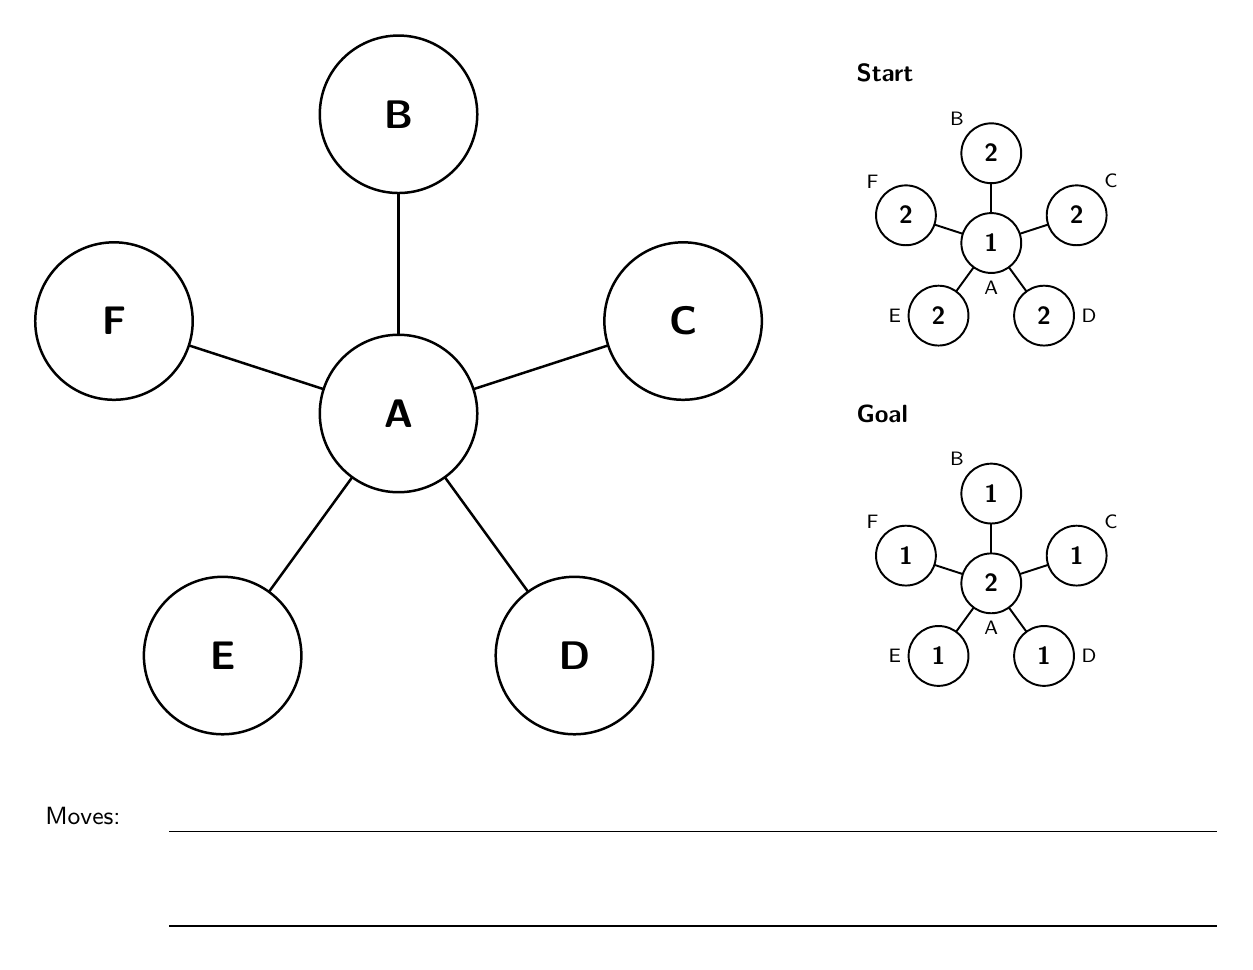
\begin{tikzpicture}[x=1mm, y=1mm]
\useasboundingbox (-47.1,-67.1) rectangle (104.9,49.0);
\draw[line width=0.9pt] (0.00,0.00) -- (0.00,38.00);
\draw[line width=0.9pt] (0.00,0.00) -- (36.14,11.74);
\draw[line width=0.9pt] (0.00,0.00) -- (22.34,-30.74);
\draw[line width=0.9pt] (0.00,0.00) -- (-22.34,-30.74);
\draw[line width=0.9pt] (0.00,0.00) -- (-36.14,11.74);
\draw[line width=0.9pt, fill=white] (0.00,0.00) circle (10.0mm);
\node[font=\Large\bfseries] at (0.00,0.00) {A};
\draw[line width=0.9pt, fill=white] (0.00,38.00) circle (10.0mm);
\node[font=\Large\bfseries] at (0.00,38.00) {B};
\draw[line width=0.9pt, fill=white] (36.14,11.74) circle (10.0mm);
\node[font=\Large\bfseries] at (36.14,11.74) {C};
\draw[line width=0.9pt, fill=white] (22.34,-30.74) circle (10.0mm);
\node[font=\Large\bfseries] at (22.34,-30.74) {D};
\draw[line width=0.9pt, fill=white] (-22.34,-30.74) circle (10.0mm);
\node[font=\Large\bfseries] at (-22.34,-30.74) {E};
\draw[line width=0.9pt, fill=white] (-36.14,11.74) circle (10.0mm);
\node[font=\Large\bfseries] at (-36.14,11.74) {F};
\node[anchor=north west, font=\small\bfseries, inner sep=0] at (58.1,44.4) {Start};
\draw[line width=0.7pt] (75.28,21.65) -- (75.28,33.05);
\draw[line width=0.7pt] (75.28,21.65) -- (86.12,25.17);
\draw[line width=0.7pt] (75.28,21.65) -- (81.98,12.43);
\draw[line width=0.7pt] (75.28,21.65) -- (68.58,12.43);
\draw[line width=0.7pt] (75.28,21.65) -- (64.44,25.17);
\draw[line width=0.7pt, fill=white] (75.28,21.65) circle (3.8mm);
\node[font=\small\bfseries] at (75.28,21.65) {1};
\node[font=\scriptsize, inner sep=0.4mm, anchor=90] at (75.28,17.35) {A};
\draw[line width=0.7pt, fill=white] (75.28,33.05) circle (3.8mm);
\node[font=\small\bfseries] at (75.28,33.05) {2};
\node[font=\scriptsize, inner sep=0.4mm, anchor=315] at (72.24,36.09) {B};
\draw[line width=0.7pt, fill=white] (86.12,25.17) circle (3.8mm);
\node[font=\small\bfseries] at (86.12,25.17) {2};
\node[font=\scriptsize, inner sep=0.4mm, anchor=225] at (89.16,28.21) {C};
\draw[line width=0.7pt, fill=white] (81.98,12.43) circle (3.8mm);
\node[font=\small\bfseries] at (81.98,12.43) {2};
\node[font=\scriptsize, inner sep=0.4mm, anchor=180] at (86.28,12.43) {D};
\draw[line width=0.7pt, fill=white] (68.58,12.43) circle (3.8mm);
\node[font=\small\bfseries] at (68.58,12.43) {2};
\node[font=\scriptsize, inner sep=0.4mm, anchor=0] at (64.28,12.43) {E};
\draw[line width=0.7pt, fill=white] (64.44,25.17) circle (3.8mm);
\node[font=\small\bfseries] at (64.44,25.17) {2};
\node[font=\scriptsize, inner sep=0.4mm, anchor=315] at (61.40,28.21) {F};
\node[anchor=north west, font=\small\bfseries, inner sep=0] at (58.1,1.1) {Goal};
\draw[line width=0.7pt] (75.28,-21.57) -- (75.28,-10.17);
\draw[line width=0.7pt] (75.28,-21.57) -- (86.12,-18.05);
\draw[line width=0.7pt] (75.28,-21.57) -- (81.98,-30.79);
\draw[line width=0.7pt] (75.28,-21.57) -- (68.58,-30.79);
\draw[line width=0.7pt] (75.28,-21.57) -- (64.44,-18.05);
\draw[line width=0.7pt, fill=white] (75.28,-21.57) circle (3.8mm);
\node[font=\small\bfseries] at (75.28,-21.57) {2};
\node[font=\scriptsize, inner sep=0.4mm, anchor=90] at (75.28,-25.87) {A};
\draw[line width=0.7pt, fill=white] (75.28,-10.17) circle (3.8mm);
\node[font=\small\bfseries] at (75.28,-10.17) {1};
\node[font=\scriptsize, inner sep=0.4mm, anchor=315] at (72.24,-7.13) {B};
\draw[line width=0.7pt, fill=white] (86.12,-18.05) circle (3.8mm);
\node[font=\small\bfseries] at (86.12,-18.05) {1};
\node[font=\scriptsize, inner sep=0.4mm, anchor=225] at (89.16,-15.01) {C};
\draw[line width=0.7pt, fill=white] (81.98,-30.79) circle (3.8mm);
\node[font=\small\bfseries] at (81.98,-30.79) {1};
\node[font=\scriptsize, inner sep=0.4mm, anchor=180] at (86.28,-30.79) {D};
\draw[line width=0.7pt, fill=white] (68.58,-30.79) circle (3.8mm);
\node[font=\small\bfseries] at (68.58,-30.79) {1};
\node[font=\scriptsize, inner sep=0.4mm, anchor=0] at (64.28,-30.79) {E};
\draw[line width=0.7pt, fill=white] (64.44,-18.05) circle (3.8mm);
\node[font=\small\bfseries] at (64.44,-18.05) {1};
\node[font=\scriptsize, inner sep=0.4mm, anchor=315] at (61.40,-15.01) {F};
\node[anchor=west, font=\small] at (-46.1,-51.1) {Moves:};
\draw[line width=0.5pt] (-29.1,-53.1) -- (103.9,-53.1);
\node[anchor=west, font=\small] at (-46.1,-63.1) {};
\draw[line width=0.5pt] (-29.1,-65.1) -- (103.9,-65.1);
\end{tikzpicture}}\par
\newpage
\textbf{Problem 7:} Using only the counters shown, can you change Start into Goal? Write the fewest moves you can find, or explain why it can't be done.\par
\vspace{10mm}
\noindent\makebox[\linewidth][c]{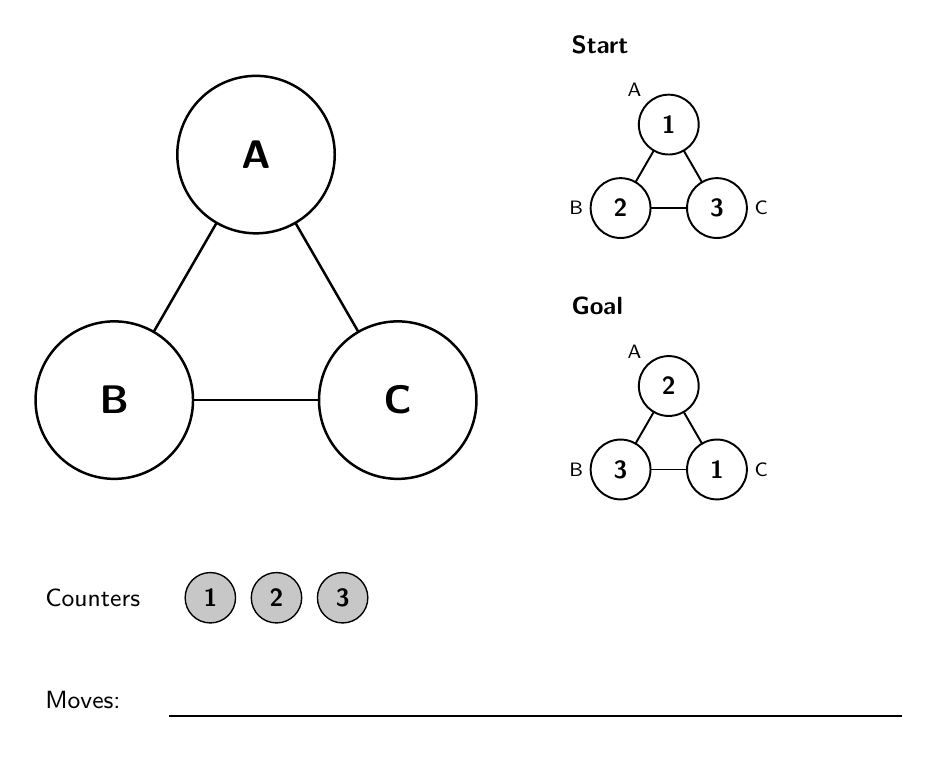
\begin{tikzpicture}[x=1mm, y=1mm]
\useasboundingbox (-29.0,-42.1) rectangle (83.0,47.3);
\draw[line width=0.9pt] (0.00,31.18) -- (-18.00,0.00);
\draw[line width=0.9pt] (-18.00,0.00) -- (18.00,0.00);
\draw[line width=0.9pt] (18.00,0.00) -- (0.00,31.18);
\draw[line width=0.9pt, fill=white] (0.00,31.18) circle (10.0mm);
\node[font=\Large\bfseries] at (0.00,31.18) {A};
\draw[line width=0.9pt, fill=white] (-18.00,0.00) circle (10.0mm);
\node[font=\Large\bfseries] at (-18.00,0.00) {B};
\draw[line width=0.9pt, fill=white] (18.00,0.00) circle (10.0mm);
\node[font=\Large\bfseries] at (18.00,0.00) {C};
\node[anchor=north west, font=\small\bfseries, inner sep=0] at (40.0,46.3) {Start};
\draw[line width=0.7pt] (52.42,34.99) -- (46.30,24.39);
\draw[line width=0.7pt] (46.30,24.39) -- (58.54,24.39);
\draw[line width=0.7pt] (58.54,24.39) -- (52.42,34.99);
\draw[line width=0.7pt, fill=white] (52.42,34.99) circle (3.8mm);
\node[font=\small\bfseries] at (52.42,34.99) {1};
\node[font=\scriptsize, inner sep=0.4mm, anchor=315] at (49.38,38.03) {A};
\draw[line width=0.7pt, fill=white] (46.30,24.39) circle (3.8mm);
\node[font=\small\bfseries] at (46.30,24.39) {2};
\node[font=\scriptsize, inner sep=0.4mm, anchor=0] at (42.00,24.39) {B};
\draw[line width=0.7pt, fill=white] (58.54,24.39) circle (3.8mm);
\node[font=\small\bfseries] at (58.54,24.39) {3};
\node[font=\scriptsize, inner sep=0.4mm, anchor=180] at (62.84,24.39) {C};
\node[anchor=north west, font=\small\bfseries, inner sep=0] at (40.0,13.1) {Goal};
\draw[line width=0.7pt] (52.42,1.79) -- (46.30,-8.81);
\draw[line width=0.7pt] (46.30,-8.81) -- (58.54,-8.81);
\draw[line width=0.7pt] (58.54,-8.81) -- (52.42,1.79);
\draw[line width=0.7pt, fill=white] (52.42,1.79) circle (3.8mm);
\node[font=\small\bfseries] at (52.42,1.79) {2};
\node[font=\scriptsize, inner sep=0.4mm, anchor=315] at (49.38,4.83) {A};
\draw[line width=0.7pt, fill=white] (46.30,-8.81) circle (3.8mm);
\node[font=\small\bfseries] at (46.30,-8.81) {3};
\node[font=\scriptsize, inner sep=0.4mm, anchor=0] at (42.00,-8.81) {B};
\draw[line width=0.7pt, fill=white] (58.54,-8.81) circle (3.8mm);
\node[font=\small\bfseries] at (58.54,-8.81) {1};
\node[font=\scriptsize, inner sep=0.4mm, anchor=180] at (62.84,-8.81) {C};
\node[anchor=west, font=\small] at (-28.0,-25.1) {Counters};
\draw[line width=0.5pt, fill=black!22] (-5.8,-25.1) circle (3.2mm);
\node[font=\small\bfseries] at (-5.8,-25.1) {1};
\draw[line width=0.5pt, fill=black!22] (2.6,-25.1) circle (3.2mm);
\node[font=\small\bfseries] at (2.6,-25.1) {2};
\draw[line width=0.5pt, fill=black!22] (11.0,-25.1) circle (3.2mm);
\node[font=\small\bfseries] at (11.0,-25.1) {3};
\node[anchor=west, font=\small] at (-28.0,-38.1) {Moves:};
\draw[line width=0.5pt] (-11.0,-40.1) -- (82.0,-40.1);
\end{tikzpicture}}\par
\vspace{18mm}
\noindent\makebox[\linewidth][c]{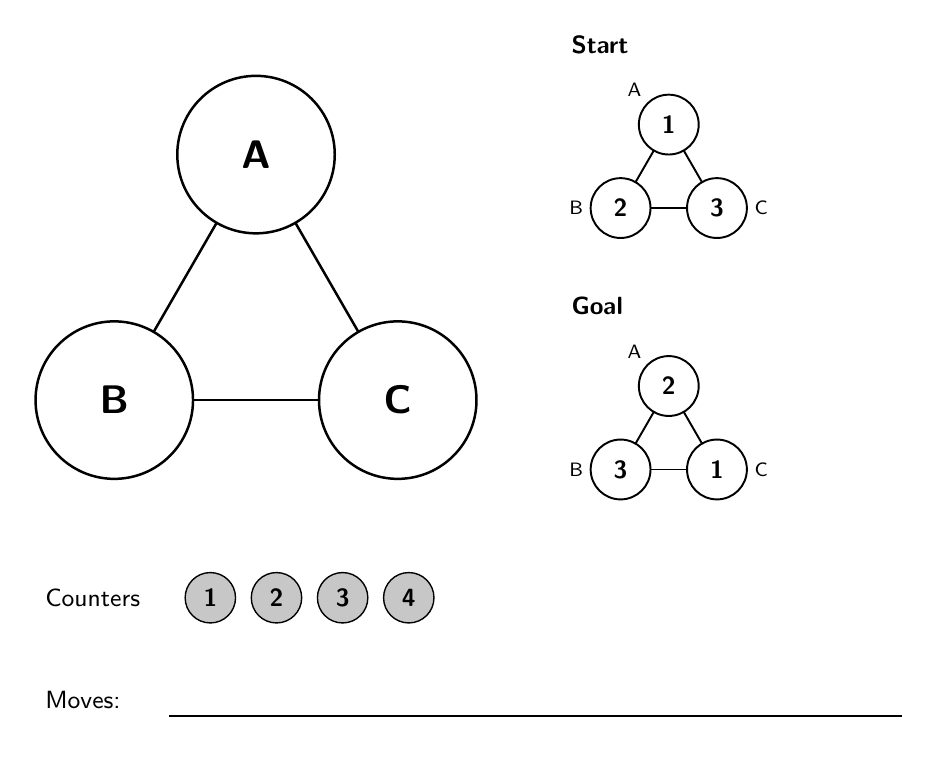
\begin{tikzpicture}[x=1mm, y=1mm]
\useasboundingbox (-29.0,-42.1) rectangle (83.0,47.3);
\draw[line width=0.9pt] (0.00,31.18) -- (-18.00,0.00);
\draw[line width=0.9pt] (-18.00,0.00) -- (18.00,0.00);
\draw[line width=0.9pt] (18.00,0.00) -- (0.00,31.18);
\draw[line width=0.9pt, fill=white] (0.00,31.18) circle (10.0mm);
\node[font=\Large\bfseries] at (0.00,31.18) {A};
\draw[line width=0.9pt, fill=white] (-18.00,0.00) circle (10.0mm);
\node[font=\Large\bfseries] at (-18.00,0.00) {B};
\draw[line width=0.9pt, fill=white] (18.00,0.00) circle (10.0mm);
\node[font=\Large\bfseries] at (18.00,0.00) {C};
\node[anchor=north west, font=\small\bfseries, inner sep=0] at (40.0,46.3) {Start};
\draw[line width=0.7pt] (52.42,34.99) -- (46.30,24.39);
\draw[line width=0.7pt] (46.30,24.39) -- (58.54,24.39);
\draw[line width=0.7pt] (58.54,24.39) -- (52.42,34.99);
\draw[line width=0.7pt, fill=white] (52.42,34.99) circle (3.8mm);
\node[font=\small\bfseries] at (52.42,34.99) {1};
\node[font=\scriptsize, inner sep=0.4mm, anchor=315] at (49.38,38.03) {A};
\draw[line width=0.7pt, fill=white] (46.30,24.39) circle (3.8mm);
\node[font=\small\bfseries] at (46.30,24.39) {2};
\node[font=\scriptsize, inner sep=0.4mm, anchor=0] at (42.00,24.39) {B};
\draw[line width=0.7pt, fill=white] (58.54,24.39) circle (3.8mm);
\node[font=\small\bfseries] at (58.54,24.39) {3};
\node[font=\scriptsize, inner sep=0.4mm, anchor=180] at (62.84,24.39) {C};
\node[anchor=north west, font=\small\bfseries, inner sep=0] at (40.0,13.1) {Goal};
\draw[line width=0.7pt] (52.42,1.79) -- (46.30,-8.81);
\draw[line width=0.7pt] (46.30,-8.81) -- (58.54,-8.81);
\draw[line width=0.7pt] (58.54,-8.81) -- (52.42,1.79);
\draw[line width=0.7pt, fill=white] (52.42,1.79) circle (3.8mm);
\node[font=\small\bfseries] at (52.42,1.79) {2};
\node[font=\scriptsize, inner sep=0.4mm, anchor=315] at (49.38,4.83) {A};
\draw[line width=0.7pt, fill=white] (46.30,-8.81) circle (3.8mm);
\node[font=\small\bfseries] at (46.30,-8.81) {3};
\node[font=\scriptsize, inner sep=0.4mm, anchor=0] at (42.00,-8.81) {B};
\draw[line width=0.7pt, fill=white] (58.54,-8.81) circle (3.8mm);
\node[font=\small\bfseries] at (58.54,-8.81) {1};
\node[font=\scriptsize, inner sep=0.4mm, anchor=180] at (62.84,-8.81) {C};
\node[anchor=west, font=\small] at (-28.0,-25.1) {Counters};
\draw[line width=0.5pt, fill=black!22] (-5.8,-25.1) circle (3.2mm);
\node[font=\small\bfseries] at (-5.8,-25.1) {1};
\draw[line width=0.5pt, fill=black!22] (2.6,-25.1) circle (3.2mm);
\node[font=\small\bfseries] at (2.6,-25.1) {2};
\draw[line width=0.5pt, fill=black!22] (11.0,-25.1) circle (3.2mm);
\node[font=\small\bfseries] at (11.0,-25.1) {3};
\draw[line width=0.5pt, fill=black!22] (19.4,-25.1) circle (3.2mm);
\node[font=\small\bfseries] at (19.4,-25.1) {4};
\node[anchor=west, font=\small] at (-28.0,-38.1) {Moves:};
\draw[line width=0.5pt] (-11.0,-40.1) -- (82.0,-40.1);
\end{tikzpicture}}\par
\newpage
\textbf{Problem 8:} Use counters 1, 2 and 3. On which of these rings can you place counters, with different numbers at the two ends of every line, so that no counter can move?\par
\vspace{10mm}
\noindent\makebox[\linewidth][s]{\hfill 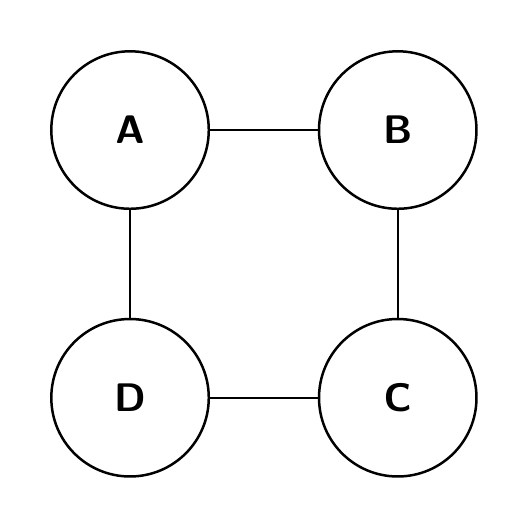
\begin{tikzpicture}[x=1mm, y=1mm]
\useasboundingbox (-30.0,-30.0) rectangle (30.0,30.0);
\draw[line width=0.9pt] (-17.00,17.00) -- (17.00,17.00);
\draw[line width=0.9pt] (17.00,17.00) -- (17.00,-17.00);
\draw[line width=0.9pt] (17.00,-17.00) -- (-17.00,-17.00);
\draw[line width=0.9pt] (-17.00,-17.00) -- (-17.00,17.00);
\draw[line width=0.9pt, fill=white] (-17.00,17.00) circle (10.0mm);
\node[font=\Large\bfseries] at (-17.00,17.00) {A};
\draw[line width=0.9pt, fill=white] (17.00,17.00) circle (10.0mm);
\node[font=\Large\bfseries] at (17.00,17.00) {B};
\draw[line width=0.9pt, fill=white] (17.00,-17.00) circle (10.0mm);
\node[font=\Large\bfseries] at (17.00,-17.00) {C};
\draw[line width=0.9pt, fill=white] (-17.00,-17.00) circle (10.0mm);
\node[font=\Large\bfseries] at (-17.00,-17.00) {D};
\end{tikzpicture} \hfill 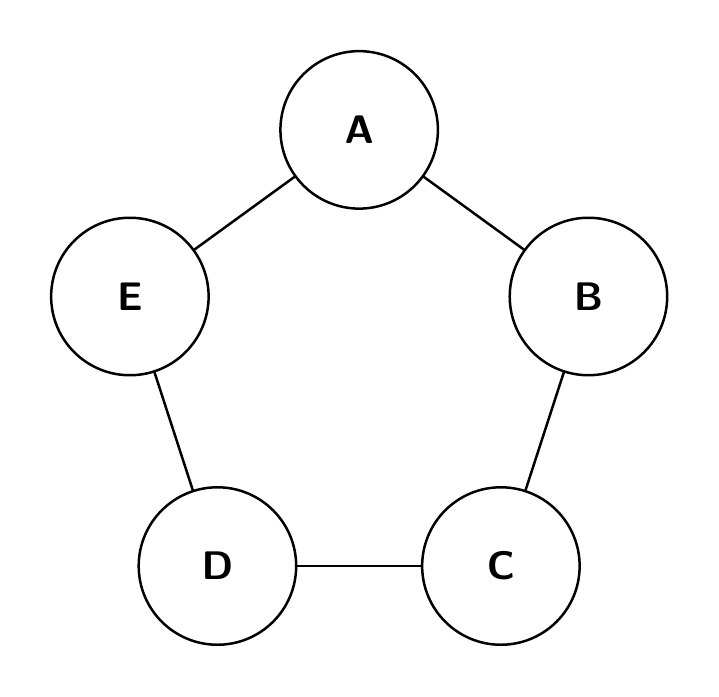
\begin{tikzpicture}[x=1mm, y=1mm]
\useasboundingbox (-42.1,-37.8) rectangle (42.1,43.6);
\draw[line width=0.9pt] (0.00,30.62) -- (29.12,9.46);
\draw[line width=0.9pt] (29.12,9.46) -- (18.00,-24.77);
\draw[line width=0.9pt] (18.00,-24.77) -- (-18.00,-24.77);
\draw[line width=0.9pt] (-18.00,-24.77) -- (-29.12,9.46);
\draw[line width=0.9pt] (-29.12,9.46) -- (0.00,30.62);
\draw[line width=0.9pt, fill=white] (0.00,30.62) circle (10.0mm);
\node[font=\Large\bfseries] at (0.00,30.62) {A};
\draw[line width=0.9pt, fill=white] (29.12,9.46) circle (10.0mm);
\node[font=\Large\bfseries] at (29.12,9.46) {B};
\draw[line width=0.9pt, fill=white] (18.00,-24.77) circle (10.0mm);
\node[font=\Large\bfseries] at (18.00,-24.77) {C};
\draw[line width=0.9pt, fill=white] (-18.00,-24.77) circle (10.0mm);
\node[font=\Large\bfseries] at (-18.00,-24.77) {D};
\draw[line width=0.9pt, fill=white] (-29.12,9.46) circle (10.0mm);
\node[font=\Large\bfseries] at (-29.12,9.46) {E};
\end{tikzpicture} \hfill}\par
\vspace{12mm}
\noindent\makebox[\linewidth][s]{\hfill 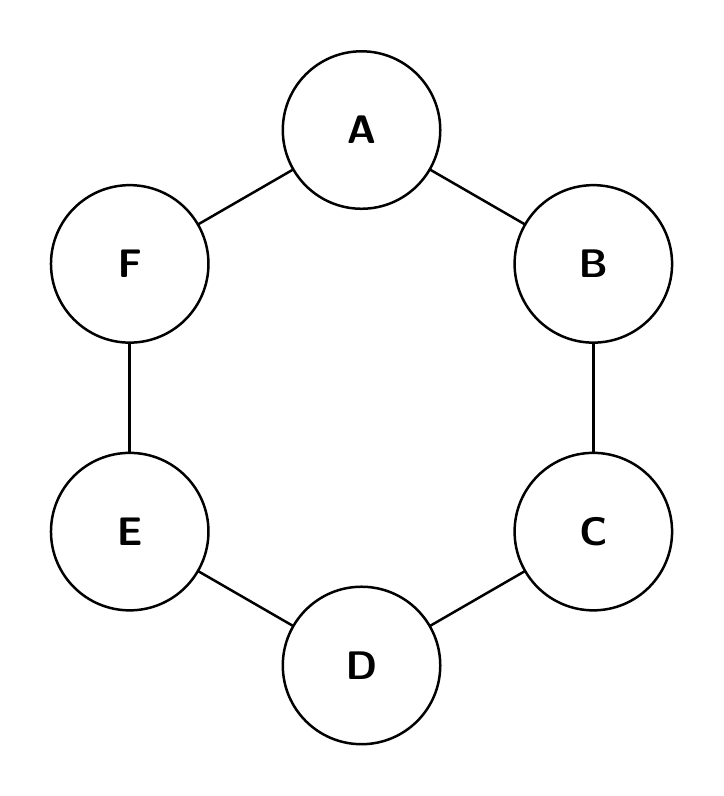
\begin{tikzpicture}[x=1mm, y=1mm]
\useasboundingbox (-42.4,-47.0) rectangle (42.4,47.0);
\draw[line width=0.9pt] (0.00,34.00) -- (29.44,17.00);
\draw[line width=0.9pt] (29.44,17.00) -- (29.44,-17.00);
\draw[line width=0.9pt] (29.44,-17.00) -- (0.00,-34.00);
\draw[line width=0.9pt] (0.00,-34.00) -- (-29.44,-17.00);
\draw[line width=0.9pt] (-29.44,-17.00) -- (-29.44,17.00);
\draw[line width=0.9pt] (-29.44,17.00) -- (0.00,34.00);
\draw[line width=0.9pt, fill=white] (0.00,34.00) circle (10.0mm);
\node[font=\Large\bfseries] at (0.00,34.00) {A};
\draw[line width=0.9pt, fill=white] (29.44,17.00) circle (10.0mm);
\node[font=\Large\bfseries] at (29.44,17.00) {B};
\draw[line width=0.9pt, fill=white] (29.44,-17.00) circle (10.0mm);
\node[font=\Large\bfseries] at (29.44,-17.00) {C};
\draw[line width=0.9pt, fill=white] (0.00,-34.00) circle (10.0mm);
\node[font=\Large\bfseries] at (0.00,-34.00) {D};
\draw[line width=0.9pt, fill=white] (-29.44,-17.00) circle (10.0mm);
\node[font=\Large\bfseries] at (-29.44,-17.00) {E};
\draw[line width=0.9pt, fill=white] (-29.44,17.00) circle (10.0mm);
\node[font=\Large\bfseries] at (-29.44,17.00) {F};
\end{tikzpicture} \hfill 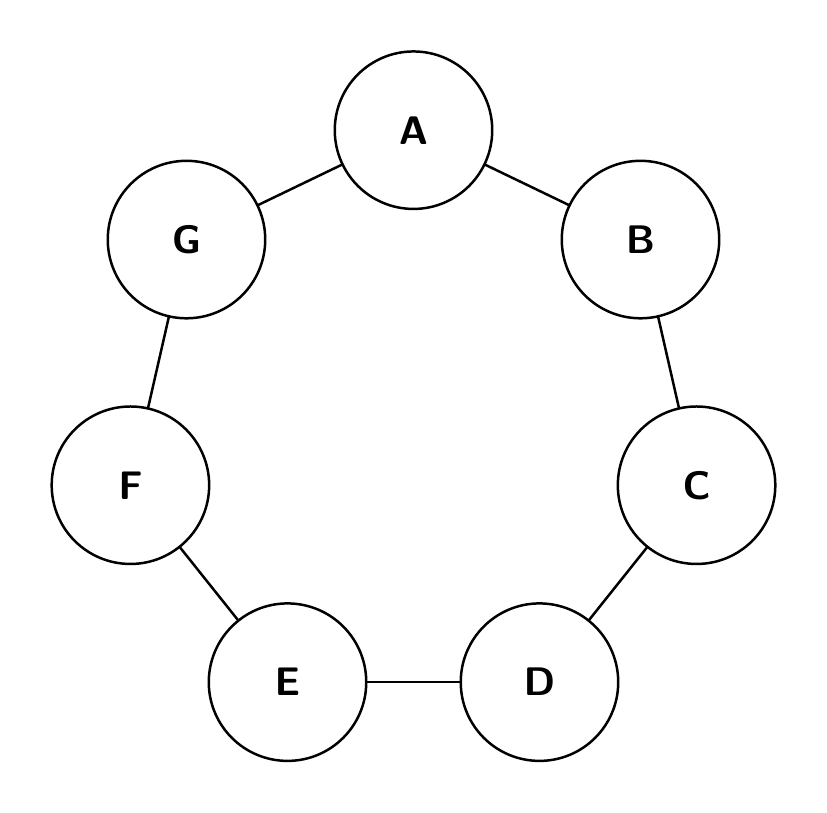
\begin{tikzpicture}[x=1mm, y=1mm]
\useasboundingbox (-49.0,-46.2) rectangle (49.0,49.9);
\draw[line width=0.9pt] (0.00,36.88) -- (28.83,22.99);
\draw[line width=0.9pt] (28.83,22.99) -- (35.95,-8.21);
\draw[line width=0.9pt] (35.95,-8.21) -- (16.00,-33.22);
\draw[line width=0.9pt] (16.00,-33.22) -- (-16.00,-33.22);
\draw[line width=0.9pt] (-16.00,-33.22) -- (-35.95,-8.21);
\draw[line width=0.9pt] (-35.95,-8.21) -- (-28.83,22.99);
\draw[line width=0.9pt] (-28.83,22.99) -- (0.00,36.88);
\draw[line width=0.9pt, fill=white] (0.00,36.88) circle (10.0mm);
\node[font=\Large\bfseries] at (0.00,36.88) {A};
\draw[line width=0.9pt, fill=white] (28.83,22.99) circle (10.0mm);
\node[font=\Large\bfseries] at (28.83,22.99) {B};
\draw[line width=0.9pt, fill=white] (35.95,-8.21) circle (10.0mm);
\node[font=\Large\bfseries] at (35.95,-8.21) {C};
\draw[line width=0.9pt, fill=white] (16.00,-33.22) circle (10.0mm);
\node[font=\Large\bfseries] at (16.00,-33.22) {D};
\draw[line width=0.9pt, fill=white] (-16.00,-33.22) circle (10.0mm);
\node[font=\Large\bfseries] at (-16.00,-33.22) {E};
\draw[line width=0.9pt, fill=white] (-35.95,-8.21) circle (10.0mm);
\node[font=\Large\bfseries] at (-35.95,-8.21) {F};
\draw[line width=0.9pt, fill=white] (-28.83,22.99) circle (10.0mm);
\node[font=\Large\bfseries] at (-28.83,22.99) {G};
\end{tikzpicture} \hfill}\par
\newpage
Lay the headers in a row, 1, 2, 3, 4, where 1 comes first. Put each card under a header, and a counter with that header's number on the card's circle. An arrow from one card to another means the first card must come earlier, under a smaller number. Cards with no arrow between them may share a header.\par
\vspace{3mm}
\noindent\makebox[\linewidth][c]{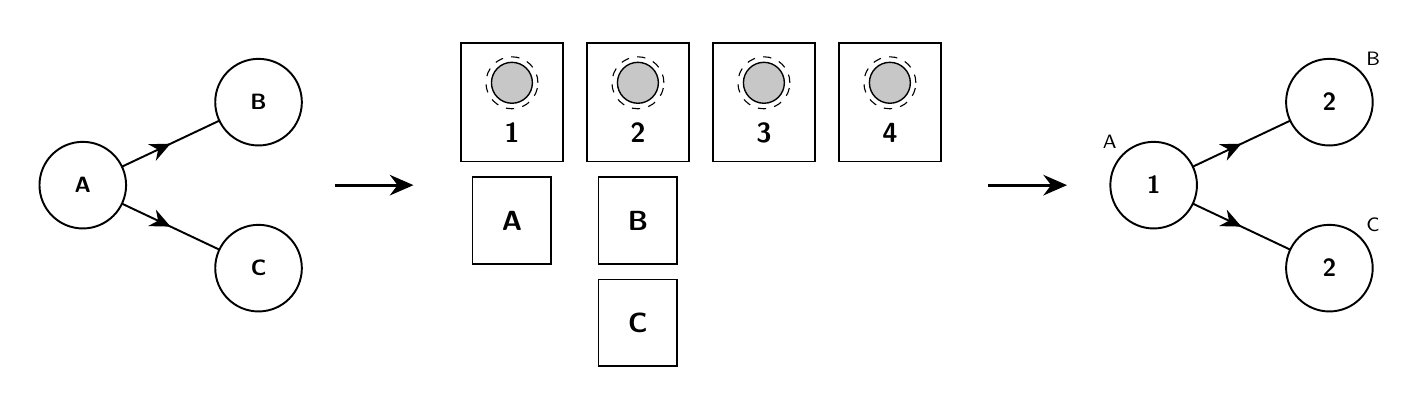
\begin{tikzpicture}[x=1mm, y=1mm]
\useasboundingbox (-7.0,-24.0) rectangle (167.0,20.0);
\draw[line width=0.7pt,smallarrow] (0.00,0.00) -- (22.32,10.54);
\draw[line width=0.7pt,smallarrow] (0.00,0.00) -- (22.32,-10.54);
\draw[line width=0.7pt, fill=white] (0.00,0.00) circle (5.5mm);
\node[font=\footnotesize\bfseries] at (0.00,0.00) {A};
\draw[line width=0.7pt, fill=white] (22.32,10.54) circle (5.5mm);
\node[font=\footnotesize\bfseries] at (22.32,10.54) {B};
\draw[line width=0.7pt, fill=white] (22.32,-10.54) circle (5.5mm);
\node[font=\footnotesize\bfseries] at (22.32,-10.54) {C};
\draw[bigarrow] (32,0) -- (42,0);
\draw[line width=0.7pt, fill=white] (48.0,3.0) rectangle (61.0,18.0);
\draw[dashed, line width=0.4pt] (54.5,13.0) circle (3.3mm);
\draw[line width=0.5pt, fill=black!22] (54.5,13.0) circle (2.6mm);
\node[font=\bfseries] at (54.5,6.6) {1};
\draw[line width=0.7pt, fill=white] (64.0,3.0) rectangle (77.0,18.0);
\draw[dashed, line width=0.4pt] (70.5,13.0) circle (3.3mm);
\draw[line width=0.5pt, fill=black!22] (70.5,13.0) circle (2.6mm);
\node[font=\bfseries] at (70.5,6.6) {2};
\draw[line width=0.7pt, fill=white] (80.0,3.0) rectangle (93.0,18.0);
\draw[dashed, line width=0.4pt] (86.5,13.0) circle (3.3mm);
\draw[line width=0.5pt, fill=black!22] (86.5,13.0) circle (2.6mm);
\node[font=\bfseries] at (86.5,6.6) {3};
\draw[line width=0.7pt, fill=white] (96.0,3.0) rectangle (109.0,18.0);
\draw[dashed, line width=0.4pt] (102.5,13.0) circle (3.3mm);
\draw[line width=0.5pt, fill=black!22] (102.5,13.0) circle (2.6mm);
\node[font=\bfseries] at (102.5,6.6) {4};
\draw[line width=0.6pt, fill=white] (49.5,-10.0) rectangle (59.5,1.0);
\node[font=\bfseries] at (54.5,-4.5) {A};
\draw[line width=0.6pt, fill=white] (65.5,-10.0) rectangle (75.5,1.0);
\node[font=\bfseries] at (70.5,-4.5) {B};
\draw[line width=0.6pt, fill=white] (65.5,-23.0) rectangle (75.5,-12.0);
\node[font=\bfseries] at (70.5,-17.5) {C};
\draw[bigarrow] (115.0,0) -- (125.0,0);
\draw[line width=0.7pt,smallarrow] (136.00,0.00) -- (158.32,10.54);
\draw[line width=0.7pt,smallarrow] (136.00,0.00) -- (158.32,-10.54);
\draw[line width=0.7pt, fill=white] (136.00,0.00) circle (5.5mm);
\node[font=\small\bfseries] at (136.00,0.00) {1};
\node[font=\scriptsize, inner sep=0.4mm, anchor=315] at (131.76,4.24) {A};
\draw[line width=0.7pt, fill=white] (158.32,10.54) circle (5.5mm);
\node[font=\small\bfseries] at (158.32,10.54) {2};
\node[font=\scriptsize, inner sep=0.4mm, anchor=225] at (162.56,14.78) {B};
\draw[line width=0.7pt, fill=white] (158.32,-10.54) circle (5.5mm);
\node[font=\small\bfseries] at (158.32,-10.54) {2};
\node[font=\scriptsize, inner sep=0.4mm, anchor=225] at (162.56,-6.30) {C};
\end{tikzpicture}}\par
\vspace{4mm}
\textbf{Problem 9:} Put every card under a header, using as few headers as you can.\par
\vspace{10mm}
\noindent\makebox[\linewidth][c]{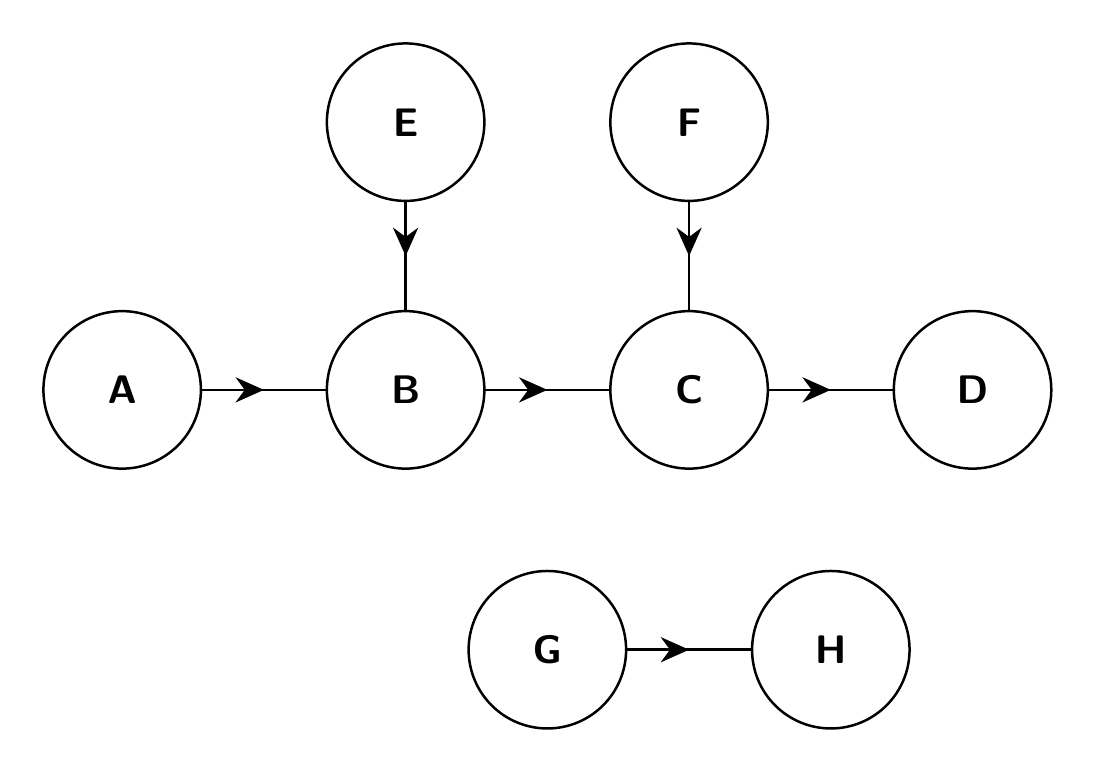
\begin{tikzpicture}[x=1mm, y=1mm]
\useasboundingbox (-12.0,-45.0) rectangle (120.0,46.0);
\draw[line width=0.9pt,midarrow] (0.00,0.00) -- (36.00,0.00);
\draw[line width=0.9pt,midarrow] (36.00,0.00) -- (72.00,0.00);
\draw[line width=0.9pt,midarrow] (72.00,0.00) -- (108.00,0.00);
\draw[line width=0.9pt,midarrow] (36.00,34.00) -- (36.00,0.00);
\draw[line width=0.9pt,midarrow] (72.00,34.00) -- (72.00,0.00);
\draw[line width=0.9pt,midarrow] (54.00,-33.00) -- (90.00,-33.00);
\draw[line width=0.9pt, fill=white] (0.00,0.00) circle (10.0mm);
\node[font=\Large\bfseries] at (0.00,0.00) {A};
\draw[line width=0.9pt, fill=white] (36.00,0.00) circle (10.0mm);
\node[font=\Large\bfseries] at (36.00,0.00) {B};
\draw[line width=0.9pt, fill=white] (72.00,0.00) circle (10.0mm);
\node[font=\Large\bfseries] at (72.00,0.00) {C};
\draw[line width=0.9pt, fill=white] (108.00,0.00) circle (10.0mm);
\node[font=\Large\bfseries] at (108.00,0.00) {D};
\draw[line width=0.9pt, fill=white] (36.00,34.00) circle (10.0mm);
\node[font=\Large\bfseries] at (36.00,34.00) {E};
\draw[line width=0.9pt, fill=white] (72.00,34.00) circle (10.0mm);
\node[font=\Large\bfseries] at (72.00,34.00) {F};
\draw[line width=0.9pt, fill=white] (54.00,-33.00) circle (10.0mm);
\node[font=\Large\bfseries] at (54.00,-33.00) {G};
\draw[line width=0.9pt, fill=white] (90.00,-33.00) circle (10.0mm);
\node[font=\Large\bfseries] at (90.00,-33.00) {H};
\end{tikzpicture}}\par
\newpage
\textbf{Problem 10:} Can the cards of each network be put under the four headers?\par
\vspace{10mm}
\noindent\makebox[\linewidth][s]{\hfill 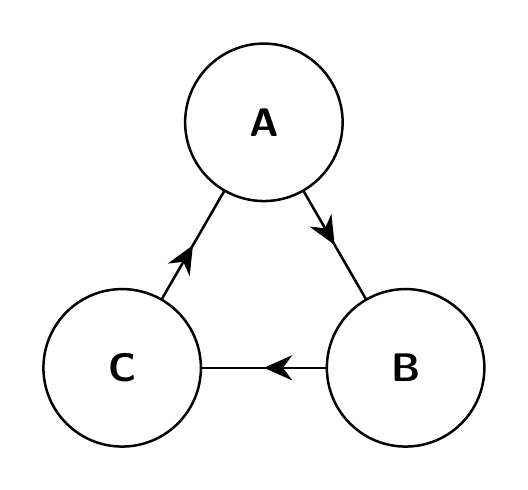
\begin{tikzpicture}[x=1mm, y=1mm]
\useasboundingbox (-30.0,-12.0) rectangle (30.0,43.2);
\draw[line width=0.9pt,midarrow] (0.00,31.18) -- (18.00,0.00);
\draw[line width=0.9pt,midarrow] (18.00,0.00) -- (-18.00,0.00);
\draw[line width=0.9pt,midarrow] (-18.00,0.00) -- (0.00,31.18);
\draw[line width=0.9pt, fill=white] (0.00,31.18) circle (10.0mm);
\node[font=\Large\bfseries] at (0.00,31.18) {A};
\draw[line width=0.9pt, fill=white] (18.00,0.00) circle (10.0mm);
\node[font=\Large\bfseries] at (18.00,0.00) {B};
\draw[line width=0.9pt, fill=white] (-18.00,0.00) circle (10.0mm);
\node[font=\Large\bfseries] at (-18.00,0.00) {C};
\end{tikzpicture} \hfill 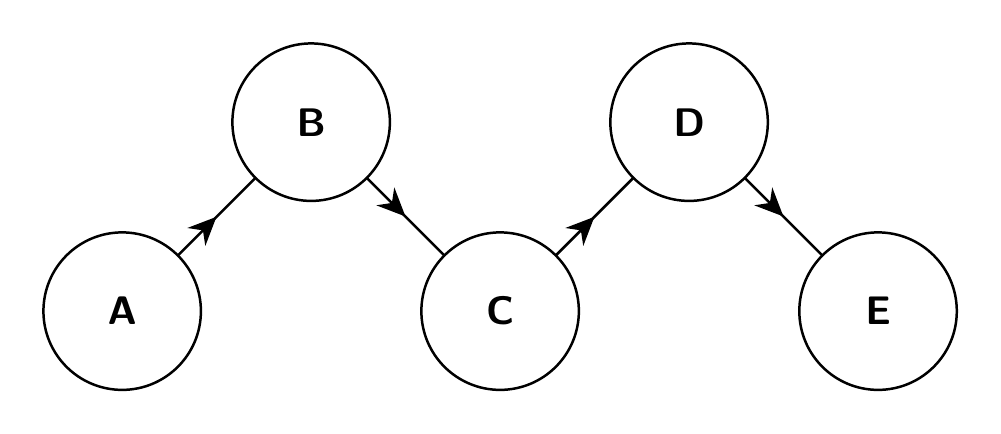
\begin{tikzpicture}[x=1mm, y=1mm]
\useasboundingbox (-12.0,-12.0) rectangle (108.0,36.0);
\draw[line width=0.9pt,midarrow] (0.00,0.00) -- (24.00,24.00);
\draw[line width=0.9pt,midarrow] (24.00,24.00) -- (48.00,0.00);
\draw[line width=0.9pt,midarrow] (48.00,0.00) -- (72.00,24.00);
\draw[line width=0.9pt,midarrow] (72.00,24.00) -- (96.00,0.00);
\draw[line width=0.9pt, fill=white] (0.00,0.00) circle (10.0mm);
\node[font=\Large\bfseries] at (0.00,0.00) {A};
\draw[line width=0.9pt, fill=white] (24.00,24.00) circle (10.0mm);
\node[font=\Large\bfseries] at (24.00,24.00) {B};
\draw[line width=0.9pt, fill=white] (48.00,0.00) circle (10.0mm);
\node[font=\Large\bfseries] at (48.00,0.00) {C};
\draw[line width=0.9pt, fill=white] (72.00,24.00) circle (10.0mm);
\node[font=\Large\bfseries] at (72.00,24.00) {D};
\draw[line width=0.9pt, fill=white] (96.00,0.00) circle (10.0mm);
\node[font=\Large\bfseries] at (96.00,0.00) {E};
\end{tikzpicture} \hfill}\par
\vspace{14mm}
\noindent\makebox[\linewidth][s]{\hfill 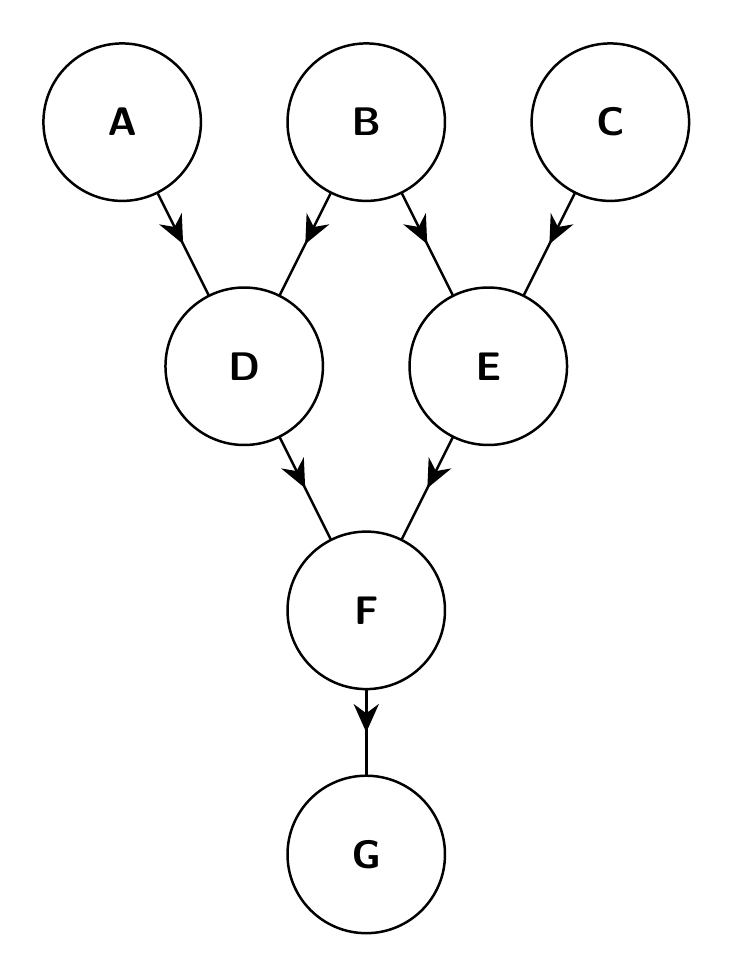
\begin{tikzpicture}[x=1mm, y=1mm]
\useasboundingbox (-12.0,-105.0) rectangle (74.0,12.0);
\draw[line width=0.9pt,midarrow] (0.00,0.00) -- (15.50,-31.00);
\draw[line width=0.9pt,midarrow] (31.00,0.00) -- (15.50,-31.00);
\draw[line width=0.9pt,midarrow] (31.00,0.00) -- (46.50,-31.00);
\draw[line width=0.9pt,midarrow] (62.00,0.00) -- (46.50,-31.00);
\draw[line width=0.9pt,midarrow] (15.50,-31.00) -- (31.00,-62.00);
\draw[line width=0.9pt,midarrow] (46.50,-31.00) -- (31.00,-62.00);
\draw[line width=0.9pt,midarrow] (31.00,-62.00) -- (31.00,-93.00);
\draw[line width=0.9pt, fill=white] (0.00,0.00) circle (10.0mm);
\node[font=\Large\bfseries] at (0.00,0.00) {A};
\draw[line width=0.9pt, fill=white] (31.00,0.00) circle (10.0mm);
\node[font=\Large\bfseries] at (31.00,0.00) {B};
\draw[line width=0.9pt, fill=white] (62.00,0.00) circle (10.0mm);
\node[font=\Large\bfseries] at (62.00,0.00) {C};
\draw[line width=0.9pt, fill=white] (15.50,-31.00) circle (10.0mm);
\node[font=\Large\bfseries] at (15.50,-31.00) {D};
\draw[line width=0.9pt, fill=white] (46.50,-31.00) circle (10.0mm);
\node[font=\Large\bfseries] at (46.50,-31.00) {E};
\draw[line width=0.9pt, fill=white] (31.00,-62.00) circle (10.0mm);
\node[font=\Large\bfseries] at (31.00,-62.00) {F};
\draw[line width=0.9pt, fill=white] (31.00,-93.00) circle (10.0mm);
\node[font=\Large\bfseries] at (31.00,-93.00) {G};
\end{tikzpicture} \hfill 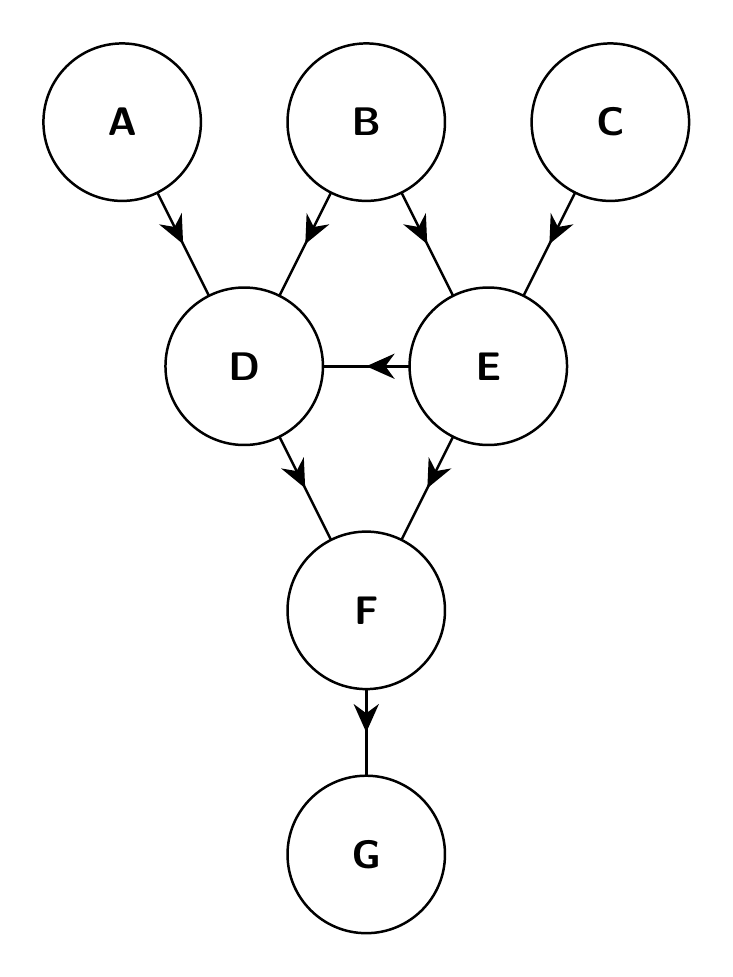
\begin{tikzpicture}[x=1mm, y=1mm]
\useasboundingbox (-12.0,-105.0) rectangle (74.0,12.0);
\draw[line width=0.9pt,midarrow] (0.00,0.00) -- (15.50,-31.00);
\draw[line width=0.9pt,midarrow] (31.00,0.00) -- (15.50,-31.00);
\draw[line width=0.9pt,midarrow] (31.00,0.00) -- (46.50,-31.00);
\draw[line width=0.9pt,midarrow] (62.00,0.00) -- (46.50,-31.00);
\draw[line width=0.9pt,midarrow] (15.50,-31.00) -- (31.00,-62.00);
\draw[line width=0.9pt,midarrow] (46.50,-31.00) -- (31.00,-62.00);
\draw[line width=0.9pt,midarrow] (31.00,-62.00) -- (31.00,-93.00);
\draw[line width=0.9pt,midarrow] (46.50,-31.00) -- (15.50,-31.00);
\draw[line width=0.9pt, fill=white] (0.00,0.00) circle (10.0mm);
\node[font=\Large\bfseries] at (0.00,0.00) {A};
\draw[line width=0.9pt, fill=white] (31.00,0.00) circle (10.0mm);
\node[font=\Large\bfseries] at (31.00,0.00) {B};
\draw[line width=0.9pt, fill=white] (62.00,0.00) circle (10.0mm);
\node[font=\Large\bfseries] at (62.00,0.00) {C};
\draw[line width=0.9pt, fill=white] (15.50,-31.00) circle (10.0mm);
\node[font=\Large\bfseries] at (15.50,-31.00) {D};
\draw[line width=0.9pt, fill=white] (46.50,-31.00) circle (10.0mm);
\node[font=\Large\bfseries] at (46.50,-31.00) {E};
\draw[line width=0.9pt, fill=white] (31.00,-62.00) circle (10.0mm);
\node[font=\Large\bfseries] at (31.00,-62.00) {F};
\draw[line width=0.9pt, fill=white] (31.00,-93.00) circle (10.0mm);
\node[font=\Large\bfseries] at (31.00,-93.00) {G};
\end{tikzpicture} \hfill}\par
\end{document}
